%% Template for EU deliverable, using the deliverable.sty style file

\documentclass[12pt,a4paper,twoside]{report}

%% common package
\usepackage[headers]{deliverable}
\usepackage{xspace}
\usepackage{verbatim}
\usepackage[usenames]{color}
\usepackage[usenames,dvipsnames]{xcolor}
%\usepackage{graphicx}
\usepackage{url}
\usepackage{array}
\usepackage{graphics} 		% for pdf, bitmapped graphics files
\usepackage{graphicx}
\usepackage{epsfig} 		% for postscript graphics files
\usepackage{epstopdf}
\usepackage{caption}
\usepackage[labelformat=simple]{subcaption}
\renewcommand\thesubfigure{(\alph{subfigure})}
\usepackage{nameref}
\usepackage{multirow}
\usepackage{color}
%\usepackage{subfigure}
%%

%%insert here other packages needed by sections
%\usepackage{esint}
\usepackage{amstext}
\usepackage{amsmath}	 	% assumes amsmath package installed
\usepackage{amssymb}  		% assumes amsmath package installed
%\renewcommand\thesubfigure{(\alph{subfigure})}
\usepackage{wrapfig}
\usepackage[]{nomencl}		% nomenclatures
\usepackage{dsfont}
%%

%%%%%%%%%%%%%%%%%%%%%%%%%%%%%% LyX specific LaTeX commands.
\newcommand{\noun}[1]{\textsc{#1}}
%% Because html converters don't know tabularnewline
\providecommand{\tabularnewline}{\\}
\renewcommand\thesubfigure{(\alph{subfigure})}

\newcommand{\figspace}{\vspace{-10pt}}
\renewcommand{\sec}{Section~}
\newcommand{\fig}{Fig.~}
\newcommand{\eq}{}
\newcommand{\app}{Appendix~}
\newcommand{\tab}{Table~}
\newcommand{\alg}{Alg.~}

\definecolor{darkgreen}{rgb}{0,0.5,0}		%Olivegreen?
\definecolor{purple}{rgb}{0.75,0,0.75}
\definecolor{pink}{rgb}{1,0.4,0.6}
%========================================================
% MATH
%--------------------------------------------------------

\renewcommand{\vec}{\boldsymbol}				% Vector
\newcommand{\mat}{\boldsymbol}					% Matrix
\DeclareMathOperator{\diag}{\mathrm{diag}} 			% Diagonal matrix

\newcommand{\R}[0]{\mathds{R}}					% Real numbers

\renewcommand{\d}{\mathrm{d}}					% Derivate
\newcommand{\gradient}{\nabla}					% Gradient
\newcommand{\hessian}{H}					% Hessian
\nomenclature{\hessian}{Hessian}

\newcommand{\inv}[0]{^{-1}} 					% Inverse
%\newcommand{\T}[0]{^T} 						% Transpose % \top
\newcommand{\T}[0]{^\top} 						% Transpose % \top

\newcommand{\norm}[1]{\left|\left| #1 \right|\right|} 		% Norm
\newcommand{\asin}[0]{\sin^{-1}} 	% 

\newcommand{\E}{\mathds{E}}	 				% expectation operator
\DeclareMathOperator{\var}{\mathrm{var}} 			% variance
\newcommand{\prob}{{p}} 					% probability density function
\newcommand{\normcdf}[1]{\Phi\left( #1 \right)} 		% Normal Cumulative distribution function
\newcommand{\normpdf}[1]{\phi\left( #1 \right)} 		% Normal probability density function
\newcommand{\gauss}[2]{\mathcal{N} \left( #1,#2 \right)}	% Gaussian Distribution


%========================================================
% MACHINE LEARNING
%--------------------------------------------------------

\newcommand{\dataset}[0]{\mathds{D}} 				% Dataset
\newcommand{\trainingset}[0]{\mathcal{D}}

\newcommand{\inputMatrix}[0]{\mat x}
\newcommand{\inputSpace}[0]{\mathcal{X}}
\newcommand{\outputMatrix}[0]{\mat y}
\newcommand{\regressionNo}[0]{f}

%========================================================
% GAUSSIAN PROCESSES
%--------------------------------------------------------

%\newcommand{\GP}[0]{\text{GP}} % Gaussian process
\newcommand{\GP}[0]{\mathcal{GP}} 	% Gaussian Process
\newcommand{\noise}[0]{w}

%========================================================
% OPTIMIZATION
%--------------------------------------------------------

\DeclareMathOperator*{\argmin}{arg\,min}
\DeclareMathOperator*{\minimize}{\text{minimize}}
\newcommand{\parameters}[0]{\vec x} 			% Parameters
\newcommand{\dimparameters}{d}					% Dimensionality parameters
\newcommand{\iteration}[0]{i}

\newcommand{\objfuncNo}[0]{f}					% Objective function
\newcommand{\objfunc}[1]{\objfuncNo\left(#1\right)}		% Objective function (as a function)
\newcommand{\respsurfNo}[0]{\hat \objfuncNo}			% Response surface
\newcommand{\respsurf}[1]{\respsurfNo \left( #1 \right)} 	% Response surface (as a function)
\newcommand{\acqfuncNo}[0]{\alpha}				% Acquisition function
\newcommand{\acqfunc}[1]{\acqfuncNo \left( #1 \right)}		% Acquisition function (as a function)
\newcommand{\acqsurf}[1]{\acqfuncNo \left( #1 \right)}		% Acquisition surface
\newcommand{\gradientline}{\d \objfunc{\parameters}/\d \parameters}

% Multi-objective optimization
\newcommand{\numbersubobj}[0]{n}
\newcommand{\mergefuncmooNo}[0]{z}
\newcommand{\mergefuncmoo}[1]{\mergefuncmooNo \left( #1 \right)}
\newcommand{\weightsmoo}[0]{\alpha}
\newcommand{\subobjfuncNo}[0]{g}
\newcommand{\subobjfunc}[1]{\subobjfuncNo \left( #1 \right)}


%========================================================
% Neural Networks
%--------------------------------------------------------

\newcommand{\nntf}[1]{\sigma \left( #1 \right)} 		% Neural Networks Transfer function
\newcommand{\nnBh}[0]{\vec {Bh}} 				% Neural Networks Bias of Hidden layer
\newcommand{\nnB}[0]{\vec B} 					% Neural Networks Bias
\newcommand{\nnW}[0]{\mat W} 					% Neural Networks Weights
\newcommand{\nnE}[0]{E} 					% Neural Networks Error function


%========================================================
% ROBOTICS
%--------------------------------------------------------

\newcommand{\q}{\mat q}
\newcommand{\dq}{\dot{\q}}
\newcommand{\ddq}{\ddot{\q}}
\newcommand{\skinInput}{\mathcal{\vec S}}

\newcommand{\frictionMatrixNo}[0]{\mat f}
\newcommand{\inertiaMatrixNo}[0]{\mat M}
\newcommand{\inertiaMatrix}[0]{\inertiaMatrixNo \left( \q \right)}
\newcommand{\gravityMatrixNo}[0]{\vec g}
\newcommand{\torque}{\tau}
\newcommand{\torques}[0]{\vec \torque}
%\newcommand{\forceNo}[0]{\vec F}
\newcommand{\extForce}[0]{\gamma}
\newcommand{\extForces}[0]{\vec \extForce}
\newcommand{\ftsForce}{F}
\newcommand{\ftsForces}{\vec \ftsForce}
\newcommand{\jtsForce}{\tau}%_text{JTS}}
\newcommand{\jtsForces}{\vec \jtsForce}%_text{JTS}}
\newcommand{\Hmatrix}[0]{\vec h \left(\q,\dq \right)}
\newcommand{\jacobian}[0]{\mat J}
\newcommand{\coriolis}[0]{C}

%========================================================
\ProcessOptions
%========================================================

\newcommand{\idyn}[0]{\textit{iDyn}}

\newcommand{\robot}{\textit{iCub}}

%==========================================
% ELMAR

\newcommand{\N}{\ensuremath{\mathcal{N}}}
\renewcommand{\vec}[1]{\ensuremath{\boldsymbol{#1}}}

%our variables used in the paper
%Initial V letter denotes the variables of the variational distribution

%model parameters followed by the variational updates
%features and covariance
\newcommand{\w}{\ensuremath{\vec w }}
\newcommand{\wi}{\ensuremath{\vec {w}^{[i]} }}
\newcommand{\Cov}{\ensuremath{\boldsymbol{\Sigma} }}
\newcommand{\Vwi}{\ensuremath{\vec \mu_{\vec {w}^{[i]}} }}
\newcommand{\VSi}{\ensuremath{\boldsymbol{\Sigma}_{\vec{w}^{[i]}} }}
%offset term
\newcommand{\wo}{\ensuremath{\vec b }}
\newcommand{\wok}{\ensuremath{\vec {b}_k }}
\newcommand{\Vwo}{\ensuremath{\vec \mu_{\vec b} }}
\newcommand{\Vwok}{\ensuremath{\vec \mu_{\vec{b}_k} }}
\newcommand{\Vlo}{\ensuremath{\sigma_{\vec b} }}
\newcommand{\Vlok}{\ensuremath{\sigma_{\vec {b}_k} }}

%loading matrix 
\newcommand{\WV}{\ensuremath{\vec M }}
\newcommand{\WVk}{\ensuremath{\vec {M}_k }}
\newcommand{\VWV}{\ensuremath{\bar{\vec M} }}
\newcommand{\VWVk}{\ensuremath{\bar{\vec{M}}_k }}

%loading matrix vectors
\newcommand{\wv}{\ensuremath{ \vec {m}^{[v]} }}
\newcommand{\wvel}[1]{\ensuremath{ \vec {m}^{[#1]} }}
\newcommand{\lv}{\ensuremath{ {\lambda^{[v]}} }}

\newcommand{\wvk}{\ensuremath{ \vec {m}^{[v]}_k }}
\newcommand{\wvi}{\ensuremath{ \vec {m}^{[v,i]} }}
\newcommand{\wvki}{\ensuremath{ \vec {m}^{[v,i]}_k }}
\newcommand{\Vwv}{\ensuremath{\vec {\mu}_{\vec{m}^{[v]}}}}
\newcommand{\Vwvel}[1]{\ensuremath{\vec {\mu}_{\vec{m}^{[#1]}}}}

\newcommand{\Vwvk}{\ensuremath{\vec {\mu}_{\vec{m}^{[v]}_k}}}
\newcommand{\Vwvkel}[1]{\ensuremath{{\vec {\mu}_{\vec{m}^{[#1]}_k}}}}
\newcommand{\Vlv}{\ensuremath{\sigma_{\vec{m}^{[v]}}}}
\newcommand{\Vlvel}[1]{\ensuremath{\sigma_{\vec{m}^{[#1]}}}}
\newcommand{\Vlvk}{\ensuremath{\sigma_{\vec{m}^{[v]}_k}}}
\newcommand{\Vlvkel}[1]{\ensuremath{\sigma_{\vec{m}^{[#1]}_k}}}
\newcommand{\VLV}{\ensuremath{\boldsymbol{\Sigma}_{\vec {M}^{[V]}}}}
\newcommand{\VLVk}{\ensuremath{\boldsymbol{\Sigma}_{\vec{M}^{[V]}_k}}}

%gamma prior on lambda
\newcommand{\VlambdaN}{\ensuremath{\bar{\lambda}^{[1:V]}} }
\newcommand{\VlambdavN}{\ensuremath{\bar{\lambda}^{[v]}} }
\newcommand{\VlambdavNk}{\ensuremath{\bar{\lambda}^{[v]}_k }}
\newcommand{\VcN}{\ensuremath{\bar{c} }}
\newcommand{\VcNk}{\ensuremath{\bar{c}_k}}
\newcommand{\VcvN}{\ensuremath{\bar{c}^{[v]} }}
\newcommand{\VcvNk}{\ensuremath{\bar{c}^{[v]}_k}}

\newcommand{\VdN}{\ensuremath{\bar{d}}}
\newcommand{\VdNk}{\ensuremath{\bar{d}_k}}
\newcommand{\VdvN}{\ensuremath{\bar{d}^{[v]} }}
\newcommand{\VdvNk}{\ensuremath{\bar{d}^{[v]}_k}}

%latent variable h
\newcommand{\hi}{\ensuremath{\vec {h}^{[i]} }}
\newcommand{\hki}{\ensuremath{\vec{h}^{[i]}_k }}
\newcommand{\Vhiv}{\ensuremath{\mu_{h^{[v,i]}} }}
\newcommand{\Vhivel}[1]{\ensuremath{\mu_{h^{[#1,i]}} }}
\newcommand{\Vhi}{\ensuremath{\vec {\mu}_{\vec {h}^{[i]}} }}
\newcommand{\Vhivk}{\ensuremath{\mu_{h^{[v,i]}_k}}}

\newcommand{\Vhik}{\ensuremath{\vec{\mu}_{\vec{h}^{[i]}_k}}}
\newcommand{\Vgi}{\ensuremath{\boldsymbol{\Sigma}_{\vec {h}^{[i]}} }}
\newcommand{\Vgik}{\ensuremath{\boldsymbol{\Sigma_{\vec{h}^{[i]}_k}}}}
\newcommand{\Vsgiv}{\ensuremath{\sigma_{h^{[v,i]}}}}
\newcommand{\Vsgivk}{\ensuremath{\sigma_{h^{[v,i]}_k}}}

%alpha
\newcommand{\ValphaN}{\ensuremath{\bar{\alpha} }}
\newcommand{\ValphaNk}{\ensuremath{\bar{\alpha}_k }}
\newcommand{\VaN}{\ensuremath{\bar{a} }}
\newcommand{\VaNk}{\ensuremath{\bar{a}_k}}

\newcommand{\VbN}{\ensuremath{\bar{b}}}
\newcommand{\VbNk}{\ensuremath{\bar{b}_k}}

%mixing coefficients
\newcommand{\Vzi}{\ensuremath{\mu_{z^{[i]}}}}
\newcommand{\Vzik}{\ensuremath{\mu_{z^{[i]}_k}}}
\newcommand{\rhoi}[1]{\ensuremath{\rho^{[i]}_{#1}}}


%%%%%%%%%%%%%%%%%%%%%%%%%%%%%% User specified LaTeX commands.
%\renewcommand{\b}[1]{\mbox{\boldmath$#1$}}
%\renewcommand{\vec}{\boldsymbol}				% Vector
%\newcommand{\mat}{\boldsymbol}					% Matrix
%%\let\vec\b
%\newcommand{\figspace}{\vspace{-10pt}}
%\newcommand{\torque}{\tau}
%\newcommand{\torques}[0]{\vec \torque}
%\newcommand{\inertiaMatrix}[0]{\inertiaMatrixNo \left( \q \right)}
%
%%\renewcommand{\columnwidth}{.5\textwidth}
%
%%ROBERTO ICRA
%\newcommand{\idyn}[0]{\textit{iDyn}}
%\newcommand{\robot}{\textit{iCub}}
%%\newcommand{\figspace}{\vspace{-10pt}}
%\newcommand{\fig}{Fig.~}
%\newcommand{\eq}{}
%\newcommand{\q}{\mat q}
%\newcommand{\dq}{\dot{\q}}
%\newcommand{\ddq}{\ddot{\q}}
%\newcommand{\Hmatrix}[0]{\vec h \left(\q,\dq \right)}
%\newcommand{\inertiaMatrixNo}[0]{\mat M}
%\newcommand{\jacobian}[0]{\mat J}
%\newcommand{\extForce}[0]{\gamma}
%\newcommand{\extForces}[0]{\vec \extForce}
%\newcommand{\T}[0]{^\top} 						% Transpose % \top
%\newcommand{\ftsForce}{F}
%\newcommand{\ftsForces}{\vec \ftsForce}
%\newcommand{\skinInput}{\mathcal{\vec S}}
%%%%%%%%%%%%%%%%%%%%%%%%%%%%%%%%%%%%%%%%%%%%%%%%%%%%%%%%%%%%%%%%%%%%%%%%%%%%%%
%%% Titlepage
%%%%%%%%%%%%%%%%%%%%%%%%%%%%%%%%%%%%%%%%%%%%%%%%%%%%%%%%%%%%%%%%%%%%%%%%%%%%%%

% declaration of variables used in style
\deliverableDocnumber{D4.2}
\deliverableTitle{Learning of tasks with multiple contacts by imitation and reinforcement learning}

\deliverableAuthor{Elmar Rueckert$^1$ and Jan Peters$^{1,2}$}
\deliverableResponsiblePartner{TUD}
\deliverableAffiliation{% Insert here authors affiliations
 $^1$ Intelligent Autonomous Systems Lab, Technische Universit\"at Darmstadt, 64289 Darmstadt, Germany.
  $^2$ Robot Learning Group, Max-Planck Institute for Intelligent Systems,
	Tuebingen, Germany.
}

\deliverableReviewer{}
\deliverableCoordinator{Jan Peters}
\deliverableActivityNumber{n} %% n=1,..,10
\deliverableActivity{Activity Name}
\deliverableDoctype{Deliverable} %% or Prototype
\deliverableClassification{Public} % or Consortium
\deliverableDistribution{Consortium} %
\deliverableStatus{Draft} % Draft or Final
\deliverableDeliveryDate{28/2/2015}
\deliverableFile{Dxx\_DeliverableName.pdf} % please do not use "-" in the name
\deliverableVersion{1.0}
\deliverableDate{Feb.~28, 2015}
\deliverableYear{2015}
\deliverablePages{\pageref{LastPage}}
\deliverableChangelog{v.0.1 & Feb 04, 2015 & Initial draft %%\\\hline
%%              v.2.0 & Feb 20, 2007 & Final version
}
\deliverableProjectStartingDate{1st March 2013}
\deliverableProjectEndDate{28th February 2017}
\deliverableProjectAcronym{CoDyCo}
\deliverableProjectTitle{Whole-Body Compliant Dynamical Contacts in Cognitive Humanoids}
 \deliverableContractNumber{600716}
 \deliverableProjectCoordinator{Istituto Italiano di Tecnologia}
 \deliverableProjectUrl{www.codyco.eu}
 \deliverableFrameworkProgramme{FP7}
 
 \deliverableWorkpackage{WP4}
 \deliverableEditors{Jan Peters and Elmar Rueckert}
 \deliverableContributors{Elmar Rueckert, Alex Paraschos, Roberto Calandra, Oliver Kroemer, Serena Invaldi, Jan Peters (TUD) / Jernej Camernik, Jan Babic (JSI)}
 \deliverableReviewers{}
\deliverableAbstract{The scope of the current deliverable is to present the results on generalizing and improving elementary tasks with contacts. 
}
\deliverableKeywordList{contacts, inverse dynamics model learning, probabilistic movement representations, reinforcement learning}


\def\BibPath{./manuscript}       % location of bibtex-files
%%%%%%%%%%%%%%%%%%%%%%%%%%%%%%%%%%%%%%%%%%%%%%%%%%%%%%%%%%%%%%%%%%%%%%%%%%%%%%
%%% Sections
%%%%%%%%%%%%%%%%%%%%%%%%%%%%%%%%%%%%%%%%%%%%%%%%%%%%%%%%%%%%%%%%%%%%%%%%%%%%%%

%% constants
\newcommand{\botegoCaps}{BOTEGO}
\newcommand{\certhCaps}{CERTH}
\newcommand{\cybionCaps}{CYBION}
\newcommand{\nuigCaps}{NUIG}
\newcommand{\ubitechCaps}{UBITECH}

%%
%%%%%%%%%%%%%%%%%%%%%%%%%%%%%% BEGIN DOCUMENT
\begin{document}

\deliverableMaketitle

%%TODO move to style
\newcolumntype{L}[1]{>{\raggedright\let\newline\\\arraybackslash\hspace{0pt}}m{#1}}
\newcolumntype{C}[1]{>{\centering\let\newline\\\arraybackslash\hspace{0pt}}m{#1}}
\newcolumntype{R}[1]{>{\raggedleft\let\newline\\\arraybackslash\hspace{0pt}}m{#1}}

\textbf{Document Revision History}
\begin{center}
\begin{tabular}{|C{2cm}|C{3cm}|p{5cm}|C{4cm}|}
\hline
\textbf{Version}&\textbf{Date}&\textbf{Description}&\textbf{Author}\\\hline
v. 0.1 & Feb. 04 & Initial Draft & Elmar Rueckert\\\hline
v. 1.0 & Feb. 28 & Final & Elmar Rueckert\\\hline
\end{tabular}
\end{center}
 
 \clearpage

\newpage
\renewcommand*\contentsname{Table of Contents}
\renewcommand*\listfigurename{Index of Figures}
\tableofcontents
\newpage
%\listoffigures
%\newpage

%%%%%%%%%%%%%%%%%%%%%%%% Start deliverable content here.

\chapter{Introduction}

This deliverable presents results of task T4.3 at the end of the second year. The achieved results are briefly discussed with respect to the task description from the Technical Annex.

\paragraph{T4.3 Generalizing and Improving Elementary Tasks with Contacts.} 
The architecture from WP3 requires a variety of tasks in order to be useful in a large number of different
scenarios. T4.3 aims at filling this void by automatically generating new tasks from data. Using both models
and data traces from WP2, elementary tasks are acquired by imitation learning and transferred to novel
situations using dynamic systems. In this case, the well-known formulation by (Ijspeert et al., 2002) will
need to be reformulated to be capable of taking contact explicitly into account. Using the recently
developed relative entropy inverse reinforcement learning techniques (Boularias et al., 2011), these tasks
can be acquired quickly while at the same time yielding an explanation of the tasks functionality in form of
an estimate of the teacher's cost function. Subsequently, the robot system will self-improve on its' current
hardware in order to achieve mastery at the task. The procedural steps of this work package are the
following:
\begin{itemize}
\item Data sets from human behavioral experiments are used to generate elementary tasks such as
reaching for objects, pushing, pulling, and standing up.

\textit{In collaboration with JSI, TUD investigated weather supporting contacts
in human arm reaching tasks are planed or an effect of a reactive controller. We
found that contacts are task related and thus planed. Further, trunk movements
are less affected by feedback compared to the lighter arms. Based on these
findings TUD will develop combined feedforward and feedback control laws and
test them on the iCub robot. A paper is currently in progress of writing.}

\item These tasks are used to instantiate an elementary task library by imitation learning, yielding both
functional elementary tasks as well as an associated cost function.

\textit{In movement libraries, a controller needs to activate suitable
primitives based on contextual cues or external events. TUD has extended their
work on probabilistic movement primitives to simultaneously learn a library of
movement primitives and control variables to activate the primitives. This work
was published at an international robotics conference \cite{Rueckert_2015} and
is discussed in Chapter \ref{sec:ElmarICRA}.}

\textit{As a first step towards understanding the stability of supporting 
contacts in humanoid robot control, TUD developed a probabilistic kernel based
model to predict the stability of object configurations. This work was published
at an international robotics conference \cite{KroemerIROS2014} and is presented
in Chapter \ref{sec:OliIROS}.}

\item The tasks are refined by reinforcement leaning such that the task will work also on the iCub despite
differences in kinematics and mechanics.
\item The task parameters of the local task are passed on to the controller from WP3.

\textit{Controller need to be able to compensate for external contact forces to
either decelerate to avoid collisions or to push objects in a controller manner,
e.g., through tactile feedback controller. TUD investigated how the tactile skin
of the iCub can be used to learn inverse dynamics models in the presence of
contacts. This work was published an international robotics conference
\cite{Calandra_ICRA15} and a pre-print is presented in Chapter
\ref{sec:RobertICRA}. In the subsequent chapter it is shown how learned  inverse
dynamics models can be used to improve torque control of the iCub. This work is
currently in progress of writing.} 



\end{itemize}

\chapter{Executive Summary}

In this deliverable, four studies relevant for improving and generalizing
elementary tasks with contacts are presented. The first work demonstrates how
multiple movement primitives as well as their activations can be learned from
human demonstrations. In a second study, TUD demonstrates how the stability of
object configurations can be modeled and used for predictions. This work will be
used in future to search for stable supporting contact configurations in
humanoid robot motions. In the last two chapters, mixtures of experts with
Gaussian processes are used to learn inverse dynamics models from tactile skins
in the iCub and how to use these models for improving the performance of torque
controller.    

%
%Oli: A kernel-based approach to
%learning object interactions from contact distributions model by Gaussians is presented. 
%This work was nominated for a best paper award at IROS 2014.


%\chapter{Are Contacts Planned in Humans? (TUD and JSI)}
%\input{elmar/HumanMotorLearningD42.tex}


\chapter{Extracting Low-Dimensional Control Variables for Movement Primitives (TUD)}\label{sec:ElmarICRA}
\begin{abstract}
Movement primitives (MPs) provide a powerful framework for data driven movement generation that
has been successfully applied for learning from demonstrations and robot reinforcement learning. 
In robotics we often want to solve a multitude of different, but related tasks. As the parameters of the primitives are typically high 
dimensional, a common practice for the generalization of movement primitives to new tasks is to 
adapt only a small set of control variables, also called meta parameters, of the primitive. Yet, for most MP representations, the encoding
of these control variables is pre-coded in the representation and can not be adapted to the considered tasks. 
In this paper, we want to learn the encoding of task-specific control variables also from data instead of relying on fixed meta-parameter representations. 
We use hierarchical Bayesian models (HBMs) to estimate a low dimensional latent variable model 
for probabilistic movement primitives (ProMPs), which is a recent movement primitive representation. We show on two real robot 
datasets that ProMPs based on HBMs outperform standard ProMPs in terms of generalization and learning from a small amount of data 
and also allows for an intuitive analysis of the movement. We also extend our HBM by a mixture model, such that we can model 
different movement types in the same dataset. 
\end{abstract}

\section{Introduction}

Movement primitives (MPs) are a compact parametric description of a movement
\cite{Paraschos2013,Ijspeert2003,Khansari-Zadeh2011,dAvella2003}. They provide a powerful framework for 
data driven movement generation as they can be learned from demonstrations as well as by reinforcement learning. They can adapt
to a new task by adapting a given set of meta-parameters
\cite{Ude2010,Kober2010, Kupcsik2013}. For example, the final joint positions or the execution speed \cite{Ijspeert2003} of the movement can be adapted. 
%\begin{figure}
\begin{wrapfigure}{r}{0.4\columnwidth}
%\vspace{-0.5em}
\begin{center}
\includegraphics[width=0.38\columnwidth]{elmarICRA/pics/IMG_1062_mod2.JPG}
\end{center}
\caption{The robot used in the experiments to learn trajectory distributions.}
\vspace{-1.5em}
%\end{figure}
\end{wrapfigure}
Yet, for most movement primitive representations, the 
set of meta-parameters is pre-coded into the movement primitive representation and can not be adapted. However, for most tasks, a different encoding of the meta-parameters
might be more appropriate than the pre-coded parameters of the primitive representation. We believe that this shortcoming has 
also hindered the application of movement primitives for more complex multi-task learning applications. In this paper we want to 
learn the encoding of the meta-parameters also from data. Our approach extracts a low-dimensional manifold in the MP parameter space. Each point 
on this manifold is described by a small set of control variables. Hence, our underlying assumption is that, while the parametrization of 
movements might be high-dimensional, useful parameter vectors for a given set of tasks typically share a lot of structure, i.e. they lie on a lower dimensional manifold.
Each demonstration can now be characterized by the corresponding 
control variables that can be seen as a compact description of the task considered in this demonstration. For example, in a table tennis scenario,
these control variables could specify the location of the hitting point or the desired return direction for the ball. 
Hence, our model can not only be applied for efficient generalization in multi-task learning with movement primitives but is also well suited 
for analyzing the movements of human demonstrators. We represent the latent manifold model by a hierarchical Bayesian model. The control
variables for each demonstrations are treated as latent variables that are also inferred from the data. The model 
is extended by a mixture model such that we can learn the control variables of multiple types of movements. We will use 
Probabilistic Movement Primitives (ProMPs)  as underlying movement primitive representation as they can be naturally integrated
in the Hierarchical Bayesian Model (HBM) representation. When learning or analyzing movement data, we have to deal
with several challenges, such as high-dimensionality, noise, missing data, partial observations, and the data can 
contain multiple modes that represent different types of movements. In order to deal with all these requirements, we 
apply a fully Bayesian approach where we integrate out all the estimated parameters of the model. In our experiments, we will
illustrate the improved generalization properties of our approach compared to the standard ProMP approach in the case of a small 
amount of training data and show how demonstrations can be easily analyzed and characterized by the extracted latent control variables. 




\subsection{Related Work}

Movement primitives can be categorized into trajectory-based
\cite{Ijspeert2003,Rozo2013,Paraschos2013} and state-based representations
\cite{Khansari-Zadeh2011}. In this paper
we will focus on trajectory based approaches as they are more commonly used and easier to scale up to higher dimensions. A common trajectory-based
approach are the dynamical movement primitives (DMPs). DMPs \cite{Ijspeert2003} are represented by a parametrized dynamical system that is given
by a linear point-attractor that is perturbed by a non-linear time dependent forcing function. The forcing function can be used to encode an arbitrary 
shape of the trajectory and the weights of the forcing function can be easily obtained from demonstrations by linear regression. One of the benefits
of the DMP approach is that it specifies a small set of meta-parameters. These meta-parameters include the final position of 
the movement, which is given by the point attractor, the final velocities, the execution speed, or the amplitude of the movement \cite{Kober2010a,Pastor2009,Ijspeert2003}. 
In multi-task learning with DMPs \cite{Kober2010,forte2012line,Kupcsik2013}, it is a common strategy to only adapt the meta-parameters 
due to the high dimensionality of the  weights of the forcing function. While DMPs have several more benefits such as stability, 
and the ability to represent stroke based and rhythmic movements, DMPs also have several limitations, such as that they can not represent optimal behavior in stochastic systems and the adaptation of the trajectory due to the meta-parameters is based on heuristics.
%, e.g., the outcome of a co-activation of DMPs or to continuously switch from one DMP to another is not predictable.
These issues have been addressed by the recently proposed Probabilistic Movement Primitives approach \cite{Paraschos2013,Paraschos2013a}. 
ProMPs estimate a distribution of trajectories instead of encoding 
single trajectories. The main benefit of the probabilistic representation is that we can use probabilistic operators such 
as conditioning for adaptation and a product of distribution for co-activating primitives. 
A distribution over trajectories also contains information on which time points are relevant for the movement, 
e.g., time points with small variance in the Cartesian end-effector space could denote task relevant via-points or targets.  
%A distribution over trajectories also contains 
%information on which time points are relevant for the movement, i.e. time points with small variance and which time points are 
%not relevant to achieve the task, i.e, time points with high variance of the joint positions. 
However, in difference to DMPs, ProMPs are lacking meta-parameters 
that can be used to adapt the trajectories with a small amount of control variables. While it would be easy to pre-specify such control variables by 
conditioning the trajectory distribution for a fixed set of time points, such an approach would again require a lot of manual tuning and is lacking flexibility. 

Our approach automatically extracts a small amount of control variables from a given set of demonstrations in the ProMP framework. 
We use a hierarchical Bayesian approach to model prior distributions, which is inspired by techniques from multi-task learning (MTL) \cite{yu05,lazaric10,daume12,ruvolo14}.
In MTL the underlying assumption is that multiple tasks (or trajectories) share a common structure, and, hence, with 
an increasing number of related tasks that have been already learned, the number of needed training samples for generalizing to a new task decreases \cite{baxter00}. 
%The main advantage of learning multiple related task together is the increased the generalization performance by exploiting the shared information \cite{caruana97, baxter97} 
%which leads to a smaller amount of required training samples. 
This property is highly desired in robotics, where the data is often high dimensional and obtaining training samples is costly.
Different approaches exist to model the shared information across tasks. They can be roughly separated into two different categories, i.e. 
methods where parameters of the model are close to each other in a geometric sense \cite{evgeniou04,ruvolo14} and approaches 
where the parameters of the model share a common structure \cite{yu05,xue07,daume09,lazaric10,rai10,passos12}. 
This structure can be a clustering assumption \cite{xue07}, a (Gaussian) prior for the parameters of all tasks \cite{yu05,lazaric10} 
or some advanced structure like the Kingman's coalescent \cite{daume09}, which is a continuous time, partitioned valued Markov process. 
Our approach is highly related to the Bayesian MTL approach presented in \cite{passos12}, 
where a prior distribution over parameters is learned. 
The prior distribution is assumed to have a low-dimensional, latent structure that is represented by a linear factor model. In 
 order to represent several modes (or non-linearities) in the data, the model is extended to a mixture model of linear factor models.
 For both, the number of mixture components and the number of factors, a non-parametric Dirichlet prior has been used.
 All parameters of the model are integrated out by the use of a combination of sampling and variational inference. 
 We will use a simplification of this model, assuming a fixed number of mixture components, without the Dirichlet priors, 
 allowing a much more efficient algorithm without the need for expensive sampling methods. 
 We extend the model of Passos et al. by an additional hyper-prior and show that this hyper-prior significantly increases the robustness of the Bayesian model.
 
\section{Probabilistic Movement Primitives}

In this section we will give a brief overview on Probabilistic Movement Primitives (ProMPs) as they provide the foundation for our hierarchical Bayesian model. 
ProMPs represent a movement by a distribution $p(\vec \tau)$ over trajectories $\vec \tau = \vec y_{1:T}$, where $\vec y_t$ specifies the joint positions (or any other quantities, 
such as a Cartesian coordinates of a ball) at time step $t$. ProMPs use a linear basis function model with $J$ basis functions to represent a single trajectory, i.e.
$$ p(\vec y_t|\vec w) = \N \left (\vec y_t \middle |\vec \Psi_t \vec w,
\beta^{-1} \vec I \right ) \textrm{ and } p(\vec \tau) = \prod_{t=1}^T
p\left(\vec y_t\middle |\vec w\right),$$
where $\beta$ denotes the precision of the data. 
The weight vector $\vec w$  is a compact representation of the trajectory. 
The basis functions $\vec \Psi_t$ only depend on the time or, alternatively, 
on the phase of the movement. For a single Degree of Freedom (DoF), $\vec \Psi_t$ is just given by a vector of normalized Gaussian basis functions $\vec \phi_t$ with 
$$ \phi_{t,i} = \frac{\exp\left(-0.5 (t - c_i)^2 \right)}{\sum_{j = 1}^J \exp\left(-0.5 (t - c_j)^2\right)},$$
where $c_i$ denotes the center of the $i$th basis function (note that to enhance readability we skipped the bandwidth parameters in this notation).

For multi-dimensional systems with $D$ DoFs, the basis function matrix
is represented by a block-diagonal matrix, i.e, 
$$\vec \Psi_t = \left[\begin{array}{cccc} \vec \phi_t^T & \vec 0^T & \dots & \vec 0^T \\ \vec 0^T & \vec \phi_t^T &  \dots & \vec 0^T \\ \vdots & \vdots & \ddots & \vdots \\ \vec 0^T & \vec 0^T & \vec 0^T & \vec \phi_t^T  \end{array}\right].$$
Due to this encoding of the basis function matrix, the trajectories of all DoFs can still be represented as 
a single weight vector $\vec w^T = [\vec w_1^T, \vec w_2^T, \dots, \vec w_D^T]$ that is given by a concatenation of all 
weight vectors for each degree of freedom.

Still, a single weight vector $\vec w$ only represents a single trajectory $\vec \tau$. In order to represent a distribution over 
trajectories $p(\vec \tau)$, we can estimate a distribution $p(\vec w)$ over the weight vectors and, subsequently, integrate out the weight vectors. 
In the original ProMP approach, a multivariate Gaussian distribution is used to model the prior distribution 
\begin{align}\label{eq:priorProMPs}
p(\vec w) = \N(\vec w| \vec \mu_w, \vec \Sigma_w). 
\end{align}
As such, the distribution over trajectories is also Gaussian and can be computed in closed form 
\begin{align*}
 p(\vec \tau) & =  \int p(\vec \tau| \vec w) p(\vec w) d\vec w, \\
 & =  \int \N\left(\vec y_{1:T}\middle| \vec \Psi_{1:T} \, \vec w, \beta^{-1}
    \vec I\right)  \N\left(\vec w\middle| \vec \mu_w, \vec \Sigma_w\right) d\vec w,  \\
  & = \N\left(\vec y_{1:T}\middle| \vec \Psi_{1:T} \, \vec w, \vec \Psi_{1:T}
    \vec \Sigma_w \vec \Psi_{1:T}^T + \beta^{-1} \vec I\right),
\end{align*}
where $\vec \Psi_{1:T}$ is a $T D \times D J$ matrix containing the basis function matrices for all time steps 
and $\vec w$ is a $D J$ dimensional column vector.

\subsection{Learning from Demonstrations with ProMPs}

A ProMP already defines a simple hierarchical Bayesian model in a similar fashion as a Bayesian linear regression model. The mean $\vec \mu_w$ 
and the covariance matrix $\vec \Sigma_w$ can be learned from data by maximum likelihood using the Expectation Maximization (EM) algorithm \cite{Dempster1977}. 
A simpler solution that works well in practice is to compute first the most likely estimate of $\vec w^{[i]}$ for each trajectory $\vec \tau^{[i]}$ independently,
 where the index $i$ denotes the $i$-th demonstration\footnote{Given a trajectory $\vec \tau_i$, the corresponding 
weight vectors $\vec w^{[i]}$ can be estimated by a straight forward least squares estimate.}. 
Subsequently, mean and covariance of $p(\vec w)$ can be estimated 
by the sample mean and sample covariance of the $\vec w^{[i]}\,$'s. 
One advantage of the EM based approach in comparison to the more direct approach is that the 
EM algorithm can also be used for learning from incomplete data where, e.g., 
some segments of the trajectories might be missing due to occlusions in vision based recordings.
%\textit{Please note that ProMPs do not require the data to be sampled at uniform time intervals as the basis function matrix 
%can be computed for continuous points in time. I am not convinced that this feature is important for us.}

However, the training of ProMPs also suffers from a severe disadvantage. As the model has a lot of parameters due
to the high-dimensional covariance matrix, ProMPs suffer from overfitting if we have little training data and noisy trajectories. 
The more sophisticated hierarchical Bayesian model for ProMPs introduced in this paper alleviates this problem. 


%\begin{figure}
%\begin{center}
%\includegraphics[width=0.8\columnwidth]{PingPong_Data.png}
%\end{center}
%\caption{(A) Trajectory prediction task on a table tennis dataset. 
%The data consists of $20$ end-effector and ball trajectories illustrated in (B). 
%(C-E) Learned distributions over trajectories for three dimensions (out of six) using ProMPs. 
%The colors (red and blue) are only used to visualize differences in the movement directions.
%\label{fig:pingpong_data_promps}
%}
%\vspace{-0.5em}
%\end{figure}

%\begin{figure*}
%\begin{center}
%\includegraphics[width=0.8\textwidth]{PingPong_Overfitting.png}
%\end{center}
%\caption{The effect of noise (A) and missing data (B) on the prediction performance of ProMPs (blue lines) and LM-ProMPs (red lines).  
%In (A), from left to right the amount of applied noise to the data is increased. 
%In (B) four different frame rates of observations ($\in \{50, 100, 200, $ and $ 300\}$ms) are investigated.
%\label{fig:pingpong_overfitting}}
%%\vspace{-0.5em}
%\end{figure*}



\subsection{Predictions with ProMPs by Conditioning}

ProMPs can also be used to predict the behavior of the demonstrator once we have seen an initial part of a new trajectory. 
Lets assume that we have observed a human demonstrator at $m=1,2, ..., M$ different time points\footnote{Note that these time points do not need to be sampled in uniform time intervals.} 
$t_1$ to $t_M$ at the positions $\vec y_{t_1}$ to $\vec y_{t_M}$. 
Let us further denote $\vec \Psi_{\vec o}$ as the concatenation of the basis function matrices for these time points 
and $\vec o$ as concatenation of the $\vec y_{t_m}$ vectors. 
Given these observations,
we can obtain a conditioned distribution $p(\vec w| \vec o)$ over the weight vectors. 
This distribution is Gaussian with mean and variance
\begin{align}
\boldsymbol{\mu}_{\vec w| \vec o} & =  \boldsymbol{\mu}_{\vec w} + \nonumber \\ 
                                  & \boldsymbol{\Sigma}_{\vec w}\boldsymbol{\Psi}_{\vec o}^T\left(\boldsymbol{\Sigma}_o + \boldsymbol{\Psi}_{\vec o}\boldsymbol{\Sigma}_{\vec w}\boldsymbol{\Psi}_{\vec o}^T\right)^{-1}\left(\vec o -\boldsymbol{\Psi}_{o}\boldsymbol{\mu}_{\vec w}\right),  \label{eq:conditioningProMP1}\\
\boldsymbol{\Sigma}_{\vec w|\vec o} & =  \boldsymbol{\Sigma}_{\vec w}-\boldsymbol{\Sigma}_{\vec w}\boldsymbol{\Psi}_{\vec o}^T\left(\boldsymbol{\Sigma}_o +\boldsymbol{\Psi}_{\vec o}\boldsymbol{\Sigma}_{\vec w}\boldsymbol{\Psi}_{\vec o}^T\right)^{-1}\boldsymbol{\Psi}_{\vec o} \boldsymbol{\Sigma}_{\vec w}. 
\label{eq:conditioningProMP2}
\end{align}
%where the matrix $\boldsymbol{\Sigma}_o$ can be used to control the importance of different dimensions.% that is in the most simple case set to $\beta^{-1}\vec I$.
The conditional distribution  $p(\vec w| \vec o)$ can be used to predict the behavior of the demonstrator for future time points $t > t_M$, 
i.e. we can determine the mean and covariance of $\vec y$ for future time points. 
Note that the same procedure can be applied for partial observations, 
where only a subset of the quantities in $\vec y_t$ is observed. 
The covariance matrix $\boldsymbol{\Sigma}_o$ can be used to control the importance of different dimensions.
%(e.g., in our experiments we will condition on reaching a desired target in the Cartesian space using a KUKA robot arm without specifying the orientation of the end-effector, i.e, via $\boldsymbol{\Sigma}_o$). 

%\section{Hierarchical Bayesian Models for Probabilistic Movement Primitives}
\section{Extracting Control Variables with Hierarchical Priors}

Our goal is to model non-linear prior distributions that can be modulated by low-dimensional latent control variables. 
We define a hierarchical prior on the weight vector $\w$ using mixture models 
\begin{align}\label{eq:priorMixture}
  p(\wi) = \sum_{k=1}^K \pi_k \N\left(\wi\middle|\wok + \WVk \hki, \alpha^{-1}
      \vec I\right).
\end{align}
The vector $\wok$ denotes an offset term and the projection matrix
$\WVk$ defines the mapping from the low-dimensional control variables 
$\hki$ to the weight vector $\wi$ of trajectory $i$. The parameter
$\alpha$ models the precision of the latent manifold priors 
and $\pi_k$ denotes the mixing coefficients.
The different mixture components can model different movement types, e.g., forehand and backhand strokes in a table tennis game. 
Within a mixture component the latent control variable $\hki$ models the adaptation of 
the movement to the current task.

All parameters of this prior distribution are unknown a priori and are learned from demonstrations.  
We follow a fully Bayesian approach, where 
we treat all parameters as random variables and introduce conjugate priors for these random variables. We 
derive variational update equations for all relevant distributions. We also demonstrate how 
predictions can be computed by conditioning with the hierarchical priors. 

We will start our discussion for the most simple case, 
using only a single mixture component. 







\subsection{Control Variables for a Single Movement Type}\label{sec:latentSingle}

For a single mixture component the prior in Eq. \eqref{eq:priorMixture} simplifies to 
\begin{align*}
p(\wi) = \N\left(\wi\middle|\wo +\WV \hi, \alpha^{-1} \vec I\right).
\end{align*}
We introduce conjugate priors for the random variables, i.e. 
we use $p(\wo) = \N(\wo|\vec 0,\vec I)$ for the offset vector, 
 $p(\hi)= \N(\hi|\vec 0,\vec I)$ for the control variables $\hi$, 
 $\alpha=\Gamma(\alpha|a_0,b_0)$ for the precision\footnote{To make this prior non-informative we use $a_0=1e-5$ and $b_0=1e-5$.} $\alpha$, 
 and $p(\WV) = \prod_v \N(\wv | \vec 0,\lv^{-1} \vec I)$ for the projection matrix $\WV$.
Here, $\wv$ denotes the $v$-th column of the matrix $\WV=[\wvel{1}, \wvel{2}, \dots, \wvel{V}]$, 
with $V$ denoting the dimensionality of the latent variable $\hi$.
The symbol $\Gamma$ denotes the Gamma distribution. 

To enhance the numerical stability of the variational updates, we also 
add a gamma prior on the precision parameters of the projection matrix, i.e. $p(\lv)=\Gamma(\lv|c_0,d_0)$. 
The influence of this additional prior is evaluated in the experimental section. 

%By using conjugate prior distributions and by assuming a fully factorized variational posterior
%closed form updates can be derived. The variational posterior reads 
As we use a variational inference approach \cite{bishop06}, we assume a complete factorization of the variational posterior given by
\begin{align*}
 q(\vec \xi) = q(\wo) q(\WV) q(\lambda_{1:V}) q(\alpha) \prod_{i=1}^L q(\wi) q(\hi) ,
\end{align*}
where $\vec \xi=\{\vec w^{[1:L]}, \vec h^{[1:L]}, \wo, \WV, \lambda_{1:V}, \alpha \}$  
and $L$ denotes the total number of demonstrations. 
The variational distributions for 
the weight vector $\wi$, 
the latent variable $\hi$, 
the offset vector $\wo$, 
the $v$-th column of the projection matrix $\WV$, 
are specified as 
$q(\wi) := \N(\wi| \Vwi, \VSi)$,
$q(\hi) := \N(\hi| \Vhi, \Vgi)$, 
$q(\wo) := \N(\wo| \Vwo, \Vlo \vec I)$, and 
$q(\wv) := \N(\wv| \Vwv, \Vlv \vec I)$. 
The remaining definitions are listed in the appendix. 

The most important variational update equations read
\begin{align*}
 \Vwi &= \VSi \left( \beta {\vec \Psi_{1:T}^{[i]}}^T \vec y_{1:T}^{[i]} +
\ValphaN \left(\Vwo + \VWV \Vhi\right)\right), \\
 \VSi &= \left(\beta {\vec \Psi_{1:T}^{[i]}}^T \vec \Psi_{1:T}^{[i]} + \ValphaN
\vec I\right)^{-1}, \\
 \Vhi &= \ValphaN \, \Vgi \, \VWV^T  \left(\Vwi - \Vwo\right), \\
\Vwo &= \Vlo \ValphaN \vec I \left(\sum_{i=1}^L \left(\Vwi - \VWV
\Vhi\right)\right), \\
\Vwv &= \Vlv \ValphaN \vec I \left(\sum_{i=1}^L \Vhiv \, \left(\Vwi -
\Vwo\right)\right),
\end{align*}
where $\VWV = [\Vwvel{1}, \dots, \Vwvel{V}]$. 
The inferred feature precision is denoted by $\ValphaN$ and 
the scalar $\Vhiv$ denotes the $v$-th element in the vector $\Vhi = [\Vhivel{1}, \dots, \Vhivel{V}]^T$.

Compared to the prior used in ProMPs in Eq. \eqref{eq:priorProMPs}, 
the combination of the latent variable $\Vhi$ 
and the projection matrix $\VWV$ implements 
a more accurate model of the prior distribution.  
As we will demonstrate, this hierarchical prior model is 
less sensitive to overfitting in the case of noisy observations 
or incomplete data. 

\subsection{Predictions by Conditioning the Hierarchical Prior}

In the hierarchical prior model, predictions are performed by computing the conditioned distribution over the latent task variable $p(\vec h| \vec o)$. 
This conditioned distribution can be simply determined by integrating out the 
weight vector $\w$
\begin{align*}
p(\vec h| \vec o) &\propto p(\vec o|\vec h) p(\vec h), \\
 =& \int_{\vec w} p\left(\vec o\middle|\vec \Psi_{\vec o}, \vec w\right)
    p\left(\vec w\middle|\vec h\right) p(\vec h) d\vec w, \\
 =& \, \N\left(\vec o\middle|\vec \Psi_{\vec o}\left(\Vwo + \VWV \vec h\right),
    \boldsymbol{\Sigma}_o  + \ValphaN^{-1} \vec \Psi_{\vec o} \vec \Psi_{\vec
    o}^T\right) p(\vec h),
 %& \N(\vec h|\boldsymbol{\mu}_{\vec h|\vec o},\boldsymbol{\Sigma}_{\vec h| \vec o}).
\end{align*}
where $p(\vec h)$ is the Gaussian prior distribution for the latent variable. 
Now, we can condition on the control variable $\vec h$ on the demonstrations to obtain a Gaussian over $\vec h$ with mean and variance
\begin{align}
 \boldsymbol{\mu}_{\vec h| \vec o} &= \VWV^T \boldsymbol{\Psi}_{\vec o}^T  \vec
    A^{-1} \left(\vec o - \boldsymbol{\Psi}_{\vec o} \Vwo \right), \label{eq:mu_o_single} \\
 \boldsymbol{\Sigma}_{\vec h|\vec o} &= \vec I - \VWV^T \boldsymbol{\Psi}_{\vec o}^T \vec A^{-1} \boldsymbol{\Psi}_{\vec o} \VWV , \label{eq:sigma_o_single}
 %\boldsymbol{\mu}_{\vec h| \vec o} &= \boldsymbol{\Psi}_{\vec o} \vec M \boldsymbol{\Sigma}_{h} (\boldsymbol{\Sigma}_o + \boldsymbol{\Psi}_{\vec o} \boldsymbol{\Sigma}_{\vec w| \vec o} \boldsymbol{\Psi}_{\vec o}^T) (\vec o - \boldsymbol{\mu}_{\vec w |\vec o})\\
 %\boldsymbol{\Sigma}_{\vec h|\vec o} &= \boldsymbol{\Sigma}_{\vec h} - \boldsymbol{\Psi}_{\vec o} \vec M \boldsymbol{\Sigma}_{\vec h} (\boldsymbol{\Sigma}_o + \boldsymbol{\Psi}_{\vec o} \boldsymbol{\Sigma}_{\vec w | \vec o} \boldsymbol{\Psi}_{\vec o}^T) (\boldsymbol{\Psi}_{\vec o} \vec  M \boldsymbol{\Sigma}_{\vec h}).
\end{align}
where $\vec A = \boldsymbol{\Sigma}_o + \boldsymbol{\Psi}_{\vec o}
\left(\ValphaN^{-1} \vec I + \VWV \VWV^T \right) \boldsymbol{\Psi}_{\vec o}^T$. 

Given the distribution over the inferred latent task variable  
the posterior over feature weights is given by 
\begin{align}
\boldsymbol{\mu}_{\vec w | \vec o} &= \Vwo + \VWV \boldsymbol{\mu}_{\vec h | \vec o}, \label{eq:post_w_single} \\
\boldsymbol{\Sigma}_{\vec w |\vec o} &= \ValphaN^{-1} \vec I + \VWV \boldsymbol{\Sigma}_{\vec h| \vec o} \VWV^T. \label{eq:post_single_sigma}
\end{align}

It is illustrative to investigate the differences of the standard conditioning of the ProMPs in Eq. \eqref{eq:conditioningProMP1} and Eq. \eqref{eq:conditioningProMP2} 
to the conditioning with the hierarchical prior. 
The conditioning in the ProMP case requires a full-rank covariance matrix, 
which is hard to obtain given a small amount of training data. 
In contrast, the latent prior model only requires the 
projection matrix $\VWV$ to perform the conditioning. 
Hence, the predictions of the latent prior model are less prone to overfitting and are, 
therefore, also applicable for a small amount of training data.

\subsection{Extension to Multiple Movement Types ($K>1$)}
\label{sec:mixmodel}

The mixture distribution in Eq. \eqref{eq:priorMixture} adds an additional multinomial variable per demonstration to our probabilistic model, 
i.e. $z^{[i]}_k \in \{0,1\}$. %This binary variable indicates to which mixture component the demonstration belongs. 
We represent this multinomial variable as binary vector $\mathbf{z}^{[i]} = \{z^{[i]}_1,...,z^{[i]}_K\}$. 

To derive variational updates, we specify a multinomial hyper-prior for the mixing indices 
$p(\vec Z) = \prod_{i=1}^L \prod_{k=1}^K (\vec \pi_k)^{z^{[i]}_k}$.

The variational updates are the same as for the case with only a single component, with 
the  difference that the trajectories are weighted by the responsibilities of the individual mixture components $\Vzik$, i.e.
\begin{align*}
    \Vwi =& \VSi \bigg( \beta {\vec \Psi_{1:T}^{[i]}}^T \vec y_{1:T}^{[i]} + \\
         & \sum_{k=1}^K \ValphaNk \Vzik \left(\Vwok + \VWVk \Vhik \right)\bigg), \\
 \VSi &= \left(\beta {\vec \Psi_{1:T}^{[i]}}^T \vec \Psi_{1:T}^{[i]} +
\sum_{k=1}^K \ValphaNk \Vzik \vec I\right)^{-1}. 
\end{align*}
Computing predictions with the mixture model is also straight forward. 
For each component we compute the conditioned distribution on the latent control variables 
as in Eq. \eqref{eq:mu_o_single} and in Eq. \eqref{eq:sigma_o_single} and 
the posterior over the feature weights using Eq. \eqref{eq:post_w_single} and Eq. \eqref{eq:post_single_sigma}.
Thereafter the posterior distributions are weighted
by the responsibilities of each mixture model   
\begin{align*}
%\boldsymbol{\hat{\Sigma}}_{\vec w |\vec o}^{[k]} &= \ValphaNk^{-1} \vec I + \VWVk \boldsymbol{\Sigma}_{\vec h| \vec o}^{[k]} \VWVk^T \\
%\boldsymbol{\hat{\mu}}_{\vec w | \vec o}^{[k]} &= \Vwok + \VWVk \boldsymbol{\mu}_{\vec h | \vec o}^{[k]}\\
z^{[k]} &= \frac{\pi_k \, \N\left(\vec o\middle|\boldsymbol{{\mu}}_{\vec w |
\vec o}^{[k]}, \boldsymbol{{\Sigma}}_{\vec w |\vec o}^{[k]}\right)}{\sum_{j=1}^K
\pi_j\N\left(\vec o\middle|\boldsymbol{{\mu}}_{\vec w | \vec o}^{[j]},
\boldsymbol{{\Sigma}}_{\vec w |\vec o}^{[j]}\right)}, \\
\boldsymbol{\Sigma}_{\vec w |\vec o} &= \sum_{k=1}^K z^{[k]} \boldsymbol{{\Sigma}}_{\vec w |\vec o}^{[k]}, \\
\boldsymbol{\mu}_{\vec w | \vec o} &= \sum_{k=1}^K z^{[k]} \boldsymbol{{\mu}}_{\vec w | \vec o}^{[k]}. 
\end{align*}
The remaining updates are listed in the appendix. 






\section{Results}

We evaluate our method on two real robot tasks. In the first task the robot
played a table tennis game and we recorded the Cartesian coordinates of a
racket mounted at its end-effector and the Cartesian coordinates of the ball. 
A Barrett WAM anthropomorphic arm was used for this experiment~\cite{Muelling2011}. 
The robot provides regular updates about its
joint positions at a rate of 1KHz that are used by the forward kinematics to
compute the Cartesian position of the racket. The ball is tracked by a
high-speed, multi-camera vision system~\cite{Lampert2012} that provides updates
at a rate of 200Hz. The extracted dataset contains twenty ball and racket
trajectories. 

In the second task we placed an obstacle in front of a KUKA lightweight arm and 
demonstrated by kinesthetic teaching different ways to approach a desired
target point in Cartesian space. During the demonstrations we avoided hitting
the obstacle and we bypassed it either by moving to the left or to the right. The
demonstrations are depicted in Fig.~\ref{fig:bimodal_data_promps}. For this
experiment we recored the Cartesian position and orientation of the
end-effector. The state vector $\vec y_t$ for this experiment is seven
dimensional, three dimensions for the position and four for the quaternion based
orientation. 

\subsection{Summary of the investigated features}

We compare the proposed model, denoted as Latent Manifold ProMPs (LMProMPs) in the figures, 
to the standard ProMP approach in the two robotic setups. 

In the table tennis
scenario we investigate the effect of noise and missing data on predicting the
final ball impact location at the opponent's side of the table and we
demonstrate how the learned latent variables can be used to semantically analyze 
the data. 

Additionally, we demonstrate the beneficial properties of the mixture model
in representing the bi-modal distribution 
required to successfully execute the KUKA reaching task. We use the learned mixture model 
to generate trajectories to new target locations, not encountered during training, and execute
them on the real robot. We demonstrate that our proposed approach
successfully avoids the obstacle, while the standard ProMPs average over the two
modes and the generalization fails.


In both experiments we used linear regression to compute the feature weights
$\vec w$ and we subsequently applied a principal component analysis. We
initialized our model with the first ten principal components.



%We evaluate the model on two kinesthetic teaching data sets, i.e., 
%in a table tennis game we recorded the Cartesian coordinates of the racket and the ball trajectories ($20$ trajectories were used).
%In a KUKA target reaching task the end-effector positions and the orientations of $28$ movements were recorded.
%In our model, the trajectories might have different time lengths but are terminated by a common event, 
%i.e., the final impact of the ball in the table tennis game that is sketched in Fig. \ref{fig:pingpong_data_promps}(A-B), 
%or when the end-effector of the KUKA arm reached the desired targets, shown in Fig. \ref{fig:bimodal_data_promps}(A-B). 
%Thus, no time alignment is needed. The progress of the movement trajectories is simply denoted by the movement phase 
%(where a phase variable of $1$ denotes the termination of the movement). 



%We initialize our model with the first ten principal components obtained in an 
%principal component analysis applied on the feature weights that were computed through 
%linear regression. In the figure legends we \textrm{LMProMPs} to denote our model that 
%represents control variables in a low-dimensional Latent Manifold.
%
%
%
%
%\subsection{Summary of the investigated features}
%
%We compare the proposed LMProMPs to the standard ProMP approach, where the table tennis data set is used to 
%investigate the effect of noise and missing data on predicting the final ball impact location. 
%Additionally, we demonstrate how the learned latent variables can be used to analyze semantically the data. 
%
%At the end of this section, we demonstrate in first experiments how the mixture model can represent bi-modal distributions 
%in the KUKA target reaching task. The learned mixture model is used to generate trajectories to new (during training unseen) 
%target location, which can be executed on the real robot. ProMPs average over the two modes and the trajectories cannot be executed on the real system. 

\subsection{The effect of noise and missing data}

%The table-tennis dataset consists of the Cartesian end-effector
%coordinates of a  Barrett WAM robotic arm and the Cartesian coordinates of the
%ball \cite{Muelling2011}. The robot data were computed using the forward
%kinematics and the ball data where gathered from a high-speed, multi-camera
%vision system \cite{Lampert2012}. The robot Cartesian position was computed at
%a rate of 1KHz using the robot's joint encoders, while the vision system was
%operating at 200Hz and provided filtered updates at a rate of 60Hz.

\begin{figure}
\begin{center}
\includegraphics[width=0.48\columnwidth]{elmarICRA/pics/PingPong_Data.png}
\end{center}
\caption{(A-B) Trajectory prediction task in a table tennis setting using $20$ end-effector and ball trajectories. 
(C-E) Learned distributions over trajectories for three dimensions (out of six) using ProMPs. 
The colors (red and blue) are only used to visualize differences in the movement directions.
\label{fig:pingpong_data_promps}
}
\vspace{-0.5em}
%\end{figure}
\end{figure}

We use the table tennis setup to predict the final impact location
of the ball at the opponent's court. We evaluate our prediction by computing the
Euclidean distance in the x,y-plane to the true impact location. The dataset
used for learning is shown in Fig. \ref{fig:pingpong_data_promps}(A-B).  It
should be noted that the colors (red and blue) in Fig.
\ref{fig:pingpong_data_promps} are only used for the visualization as no labels
were used for modeling the data. 

For a baseline comparison we trained the ProMPs on the same data. 
The learned distributions over trajectories for ProMPs are illustrated for three Cartesian coordinates in Fig.
\ref{fig:pingpong_data_promps}(C-E). We denote the mean of the trajectory
distribution with a solid black line and the standard deviation by the shaded
region. 

In the collected dataset, the robot returns the ball within $550$ms to $650$ms in
advance to the final ball impact.  In our comparison, we analyze the prediction
performance with respect to the time until the impact event, where we focus on
the movement phase right after the stroke, $\approx 625$ms before the end. We
used leave-one-out cross-validation to compute the test error.



%The goal of this task is to predict the final impact location of the ball 
%(we evaluated the Euclidean distance in the x,y-plane to the true impact location) shown in Fig. \ref{fig:pingpong_data_promps}(A-B).
%Note that the colors (red and blue) in Fig. \ref{fig:pingpong_data_promps} are only used 
%for the visualization as no labels were used for modeling the data. 
%For ProMPs the learned distributions over trajectories are illustrated 
%for three coordinates in Fig. \ref{fig:pingpong_data_promps}(C-E). 
%The mean is denoted by the solid black line and the standard deviation by the shaded region. 



%In the data, the opponent (the Barrett WAM robot arm) returns the ball within the interval $[550,650]$ms in advance to the final ball impact. 
%In our comparison, we analyze the prediction performance with respect to the time until the impact event, 
%where we focus on the movement phase right after the stroke ($\approx 625$ms). 
%Leave-one-out cross-validation was used to compute the test error.

\begin{figure*}
\begin{center}
\includegraphics[width=0.8\textwidth]{elmarICRA/pics/PingPong_Overfitting.png}
\end{center}
\caption{The effect of noise (A) and missing data (B) on the prediction performance of ProMPs (blue lines) and LM-ProMPs (red lines).  
In (A), from left to right the amount of applied noise is increased. 
In (B) four different frame rates of observations ($\in \{50, 100, 200, $ and $ 300\}$ms) are investigated.
\label{fig:pingpong_overfitting}}
%\vspace{-0.5em}
\end{figure*}

A fast multi-camera vision setup, good lighting conditions, and access to the
opponents sensor readings are amenities we can not always afford. Therefore, we
simulate the effect of noisy and incomplete observations, and we evaluate their
impact on the prediction performance. First, we add zero-mean Gaussian
observation noise to the Cartesian coordinates of the racket and to the
Cartesian coordinates of the ball. The standard deviation of the noise used in
our evaluation is $\sigma_h \in 10^{-2}\{0, 2, 4, 6\}$ and $\sigma_b \in 10^{-2}\{0, 5, 10, 15\}$
for the racket and the ball, respectively. The results are illustrated in Fig. \ref{fig:pingpong_overfitting}(A), 
where we show the advantage of the learned prior distribution using latent
variables. %ur approach out performs the original ProMPs at higher noise levels.
  
%In a realistic setting we would not have access to the sensor readings of the opponent nor an accurate and fast multi-camera vision system might be available.  
%We therefore simulate the effect of noise on the prediction performance. 
%Normal distributed Gaussian noise is added to the cartesian coordinates of the hand 
%(with a standard deviation of $\sigma_h \in 10^{-2}\{0, 2, 4, 6\}$) and to the ball trajectories (with a standard deviation of $\sigma_b \in 10^{-2}\{0, 5, 10, 15\}$). 
%The advantage of the learned prior distribution using latent variables is illustrated in Fig. \ref{fig:pingpong_overfitting}(A), 
%where in the panels from left to right the amount of added noise is linearly increased.

Additionally, we evaluate the effect of sparse observations using different sampling
intervals, $\{50, 100, 200, $ and $, 300\}$ms. The proposed model is more robust
with respect to sparse observations, whereas the standard ProMPs overfit to the
training data, especially in the early phase of the movement. The performance
comparison of the two approaches is illustrated in Fig.
\ref{fig:pingpong_overfitting}(B).

%The effect of missing data is illustrated in Fig. \ref{fig:pingpong_overfitting}(B), 
%where for the evaluations in the panels from left to right 
%observations were sampled every $\{50, 100, 200, $ and $, 300\}$ms. 
%The proposed model is robust with respect to sparse observations, 
%whereas the standard ProMPs overfit to the training data, 
%especially in the early phase of the movement. 

\subsection{Analyzing the model parameters}

As opposed to most movement primitive approaches, our model has only one free parameter to
choose that is the precision of the data denoted by $\beta$. For large $\beta$
values the number of contributing 
latent variables in the generative model is increased, and, at some point, the
model will overfit to the training data.  To analyze this effect, we approximate 
the complexity of the learned model by computing the rank of the linear feature
weights denoted by $\WV \hi$ in Eq. \eqref{eq:priorMixture}. 

\begin{figure}
\begin{center}
\includegraphics[width=0.48\columnwidth]{elmarICRA/pics/PingPong_Robustness.png}
\end{center}
\caption{(A) The data precision parameter $\beta$ can be used to adapt the model complexity while avoiding overfitting (shown in the $2$nd and $3$rd panel for two planning horizons until the ball impact). 
(B) The gamma prior on the precision parameters $\lambda$ to increase the numerical stability has little effect on the prediction performance (for $c_0 \ge 1$). 
(C) Investigation of the effect of the latent variables, where the first dimension of $\textbf{h}$ describes the slope whereas the second dimension relates to the waviness (D).
\label{fig:pingpong_model}}
%\vspace{-0.5em}
%\end{figure}
\end{figure}
%include time sync?

For values of $\beta \in \{1, 10, 50, 100, 200, 500, 1000, 5000\}$ we compute
the training and test error. The prediction
performance is shown in Fig. \ref{fig:pingpong_model}(A). The lowest test error was
achieved for $\beta=10$ (for a prediction horizon of $625$ms).  Note that the test error will not converge to zero
due to noise introduced with $\sigma_h=0.02$ and $\sigma_b = 0.05$, and the
sparse observations at $50$ms intervals.


%The proposed model has one free parameter to tune that is the precision of the data denoted by $\beta$. 
%For large $\beta$ values we \textit{trust} the training data more and the number of contributing latent variables 
%in the generative model will increase and at some point the model will overfit to the training data. 
%To analyze that effect we use a simple measure of the complexity of the learned model that is the rank of the 
%linear feature weights denoted by $\WV \hi$ in Eq. \eqref{eq:priorMixture}. 
%For the table tennis data set an evaluation of the model complexity, the training and the test error for $\beta \in \{1, 10, 50, 100, 200, 500, 1000, 5000\}$ is shown in 
%Fig. \ref{fig:pingpong_model}(A). The best test error was achieved with $\beta=10$, 
%which is illustrated in the panel on the right in Fig. \ref{fig:pingpong_model}(A). 
%Shown are the prediction errors for two different time horizons until the ball impact, 
%i.e., $625$ms (approx. at the stroke event) and $0$ms (ball impact). 
%Note that the test error will not converge to zero due to noise ($\sigma_h=0.02$ and $\sigma_b = 0.05$) and missing data ($50$ms).



The numerical stability of the LMProMPs can be increased with the addition of a gamma
prior on the $\lv$ parameters, discussed in Subsection \ref{sec:latentSingle}. 
To investigate the influence of this regularization on the test error, we evaluated
gamma priors with a constant mean ($c_0/d_0=100$) and increasing precision in
the interval $c_0\in [0.05, 500]$. For small values of $c_0$ the prior converges
to a uniform distribution. For $c_0\ge1$ the variational updates were
numerically stable and the gamma prior had only little influence on the test
error, as shown in Fig. \ref{fig:pingpong_model}(B).
  
%In Subsection \ref{sec:latentSingle} we argued that the numerical stability of the hierarchical Bayesian model 
%can be increased by adding a gamma prior 
%on the $\lv$ parameters. 
%To investigate the influence of this regularization on the test error, 
%we evaluated gamma priors with a constant mean ($c_0/d_0=100$) and increasing precision, i.e., using $c_0\in [0.05, 500]$ 
%(where for small $c_0$ values the prior converges to a uniform distribution). 
%For $c_0\ge1$ the variational updates were numerically stable and the gamma prior had only little 
%influence on the test error shown in Fig. \ref{fig:pingpong_model}(B).

Finally, we semantically analyze the table tennis dataset to evaluate how the
latent variable affect the learned prior distribution.  We trained the
model with $10$-dimensional latent variables $\hi$
in Eq. \eqref{eq:priorMixture}. The effect of the first two latent dimensions
in the generative model is illustrated in Fig. \ref{fig:pingpong_model}(C-D).
The two latent dimensions of the model affect the slope and the waviness of the
x-coordinate of the racket trajectories shown in Fig. \ref{fig:pingpong_model}(D).


\subsection{Learning bi-modal trajectory distributions}

%We evaluate the performance gain by the introduction of a mixture model on a bi-modal target-reaching task. 
To demonstrate that LMProMPs can model multi-modal distributions,  
we study demonstrations of a bi-modal target-reaching task. 
A KUKA lightweight arm was used to reach for 
different target locations on a table while avoiding an obstacle. 
We used kinesthetic teaching and we demonstrated two different ways to approach the target. The
setup and demonstrations are shown in Fig. \ref{fig:bimodal_data_promps}(A). 

\begin{figure}
%\begin{figure}%[!t]
\begin{center}
\includegraphics[width=0.48\columnwidth]{elmarICRA/pics/BiModal_Data_ProMPs.png}
\end{center}
\caption{(A) Experimental setting and two dimensions out of the $7$-dimensional dataset (three end-effector coordinates and the four dimensional quaternions). The colors (red and blue) denote the movement direction to avoid the obstacle.
(B-C) Learned distributions using ProMPs. The mean is denoted by the black line and the standard deviation by the shaded region. 
ProMPs cannot represent the bi-modal distribution in the $2$nd panel in (B) and 
the conditioning on unseen targets might fail (D). 
\label{fig:bimodal_data_promps}}
%\vspace{-0.5em}
%\end{figure}
\end{figure}

For a comparison, we trained ProMPs to learn from the demonstrations, 
which were unable to represent the two modes. 
As a result, generalization by
conditioning to not encountered target locations may result in trajectories that pass
through the obstacle. The learned distributions and example trajectories are shown in Fig. \ref{fig:bimodal_data_promps}(B-C).

%The mixture model was evaluated on a bi-modal target reaching task, 
%where through kinesthetic teaching on a KUKA arm the robot was taught to 
%reach for different target locations on a table while avoiding an obstacle, shown in Fig. \ref{fig:bimodal_data_promps}(A).
%ProMPs learn distributions that average over the two possible modes, 
%which is illustrated for the end-effector trajectories in Fig. \ref{fig:bimodal_data_promps}(B-C). 
%The two modes are denoted by the colors red and blue. 
%As shown in Fig. \ref{fig:bimodal_data_promps}(D) conditioning fails and the obstacle cannot be avoided. 
  
 
 
 
\begin{figure}
\begin{center}
\includegraphics[width=0.48\columnwidth]{elmarICRA/pics/BiModal_Mixture.png}
\end{center}
\caption{Learned bi-modal distribution (the colors red and blue denote the modes) using the proposed mixture model with two mixture components (A-B). 
The latent variable is used to specialize on subregions within the distribution of the mixture component. 
This is illustrated for two dimensions of $\textbf{h}$, where solid black lines denote the mean. 
(C) Conditioning result using LMProMPs. (D) Real robot results.
\label{fig:bimodal_mixture}}
%\vspace{-0.5em}
%\end{figure}
\end{figure}
  
In contrast, the LMProMPs model is able to capture the two modes of the
demonstrations, as shown in Fig. \ref{fig:bimodal_mixture}. We initialized the
experiment with \textit{K-means} clustering method using two components.  The
learned prior distribution and the influence of the first two dimensions of the
latent variable are illustrated in Fig. \ref{fig:bimodal_mixture}(A-B).
Each mixture component specializes on one mode of the data.  Using the learned
bi-modal prior distribution, our model is able to generate trajectories to new 
target locations that avoid the obstacle as shown in Fig.
\ref{fig:bimodal_mixture}(C).  
The inferred trajectories are smooth and can be
executed on the real robot using inverse kinematics to obtain a reference joint
trajectory and inverse dynamics control to execute it.  The resulting
trajectories of the end-effector of the real robot are illustrated in Fig.
\ref{fig:bimodal_mixture}(D). 


\section{Conclusion}
A desired feature of motor control approaches is to have a low number of 
control parameters that can be used to adapt learned skills to new or changing situations. 
In existing movement primitive approaches \cite{Paraschos2013,Ijspeert2003,Khansari-Zadeh2011} 
 these control parameters are predefined and can not adapt to the complexity of the tasks. 
In this paper we proposed a probabilistic movement primitive representation with hierarchical priors 
that learns these control parameters as well as distributions over trajectories 
from demonstrations. We demonstrated on two kinesthetic teaching datasets that 
the control variables can be used to generate new trajectories or to analyze the data. 
The model naturally extends to mixture models, where multi-modal distributions can be represented. 
In future work we will investigate non-parametric variants using, e.g., Dirichlet processes 
on more challenging simulated and real-robot tasks with a larger number of modes.



\chapter{Predicting Object Interactions from Contact Distributions (TUD)}\label{sec:OliIROS}
\section*{Abstract}
Contacts between objects play an important role in manipulation tasks.
Depending on the locations of contacts, different manipulations or
interactions can be performed with the object. By observing the contacts
between two objects, a robot can learn to detect potential interactions
between them. 

Rather than defining a set of features for modeling the contact distributions,
we propose a kernel-based approach. The contact points are first
modeled using a Gaussian distribution. The similarity between these
distributions is computed using a kernel function. The contact distributions
are then classified using kernel logistic regression. The proposed
approach was used to predict stable grasps of an elongated object,
as well as to construct towers out of assorted toy blocks. 
%\end{abstract}

\section{Introduction}

\begin{wrapfigure}{r}{0.25\columnwidth}
	\centering
	\includegraphics[width=.99\linewidth]{oli/PicsforIROS2014/RobotStacking}
	\caption{\label{fig:The-Darias-robot}The Darias robot performing a block stacking
task.}
	\figspace
%\end{figure}
\end{wrapfigure}

Manipulation tasks almost always involve direct physical contact between
two or more objects. These contacts can be between different objects
in the robot's environment, or between an object and the robot. Depending
on the locations of the contacts, different types of interactions
and manipulations can occur. For example, a contact on the side of
an object may allow for pushing and sliding the object, while a contact
on the bottom can be used for lifting or supporting the object. In
order to successfully perform a manipulation task, a robot must be
able to determine the potential interactions between objects and utilize them
to accomplish the task's goal. 

Utilizing contact information in an efficient manner is however not
a trivial task. Analytical approaches tend to require accurate models
of the objects, and rely on simplified contact models \cite{GraspSurveyBohg}.
In an effort to make robots more autonomous, learning approaches have
become more widely adopted in the field of robot manipulation \cite{objectPlacementYun,KopickiZSMW11,SimulatedAffordanceLearning}.
However, representing contacts between objects often relies on hand-crafted
features for the given task. 

In this paper, we propose an example-based learning approach to detect
interactions between objects from their contact distributions. We
pose the problem of detecting interactions as a binary classification
problem, wherein the robot has to predict whether or not a certain
interaction is occurring based on the geometry and relative poses
of the objects. The robot first computes which regions of the objects
are in contact with each other. 
The resulting cloud of contact points
is subsequently modeled as a Gaussian distribution. A Bhattacharyya
kernel function \cite{JebaraK03} can then be used to compute the
similarities between the contact distributions and, thus, classify
them using kernel logistic regression. In this manner, the robot uses
the similarity between the current contact distribution and previous
distributions in order to classify the potential interaction. The
details of the approach are explained in Section \ref{sec:Classifying-Object-Interactions}.

The proposed approach was implemented on the real robot shown in Fig.
\ref{fig:The-Darias-robot}. In the first experiment, the robot was
given the task of predicting which grasps allow it to steadily pick
up an elongated object. The second experiment required the robot to
stack assorted blocks. The details of the experiments are given in
Section \ref{sec:Experiments}.


%\begin{figure}
%\begin{centering}
%\includegraphics[width=0.445\columnwidth]{oli/PicsforIROS2014/RobotStacking}
%\par\end{centering}
%
%\caption{\label{fig:The-Darias-robot}The Darias robot performing a block stacking
%task.}
%\end{figure}



\section{Learning From Contact Distributions\label{sec:Classifying-Object-Interactions}}

In this section, we first outline related work in interaction detection.
In Sections \ref{sub:Contact-Points} to \ref{sub:Computing-Contact-Distributions},
we explain how contacts between objects are detected and used to create
contact distributions. In Sections \ref{sub:Comparing-Contact-Distributions}
to \ref{sub:Classifying-Contact-Distribution}, we provide a kernel
function for computing the similarity between contact distributions
and explain how it is used to classify the distributions using kernel
logistic regression. 


\subsection{Related Work}

\begin{figure}
\begin{centering}
\begin{tabular}{cc}
\includegraphics[width=0.23\columnwidth]{oli/PicsforIROS2014/3FingGrasp} & \includegraphics[width=0.23\columnwidth]{oli/PicsforIROS2014/4FingGrasp}\tabularnewline
3-Fingered Grasp & 4-Fingered Grasp\tabularnewline
\end{tabular}
\par\end{centering}

\caption{\label{fig:Grasp-types}The two types of grasps that were used during
the lifting experiment. The three-fingered grasp uses the tips of
the thumb, middle, and index fingers in order to pinch the object. The ring and little finger are not touching the box.
The four-fingered grasp additionally uses the back of the ring finger
on the top of the box in order to provide additional support. }
\end{figure}
Learning symbolic representations of geometric relations between objects,
e.g. object A is \noun{on} object B, is an important skill for performing
complex manipulation tasks. Rosman and Ramamoorthy \cite{ContactNetwork}
proposed the use of a contact network to learn the spatial relations
between objects. Contact points were detected using a support vector
machine to separate the point clouds of the objects. The vectors between
the objects' contact points were then computed and used to classify
relations such as \emph{on} and \emph{adjacent} using a $k$-nearest
neighbors classifier. Kulick et al. use an active learning approach
to efficiently learn a symbolic representation of the relations between
objects \cite{kulickSymbolLearning}. Using features such as the heights
of objects and the relative positions between objects, they train
a Gaussian process classifier to learn in which geometric states the
predicate is true. 

Classifying interactions between objects is also closely related to
learning affordances \cite{gibson1979}. If an object allows a robot
to perform an action with it, than the object is said to ``afford''
that action. Affordances have been widely studied in robotics \cite{ToAffordorNottoAfford,koppula2013_anticipatingactivities,MontesanoBayesNetAffordance},
and especially in the field of robot grasp synthesis \cite{GraspSurveyBohg}.
Recently, several papers have proposed template-based approaches for
detecting where an object can be grasped \cite{Herzog_AR_2013,detry2012a,Kroemer_ICRA_2012}.
These approaches predict where to grasp an object based on the local
shape of the object relative to the hand. The approach presented by
Detry et al. \cite{detry2012a} learns both the bounding box of points
to consider when comparing grasps as well as a dictionary of graspable
parts. 

Contact information can also be represented in the form of tactile
sensor readings. Bekiroglu et al. \cite{bekiroglu2011d} proposed
learning to predict stable grasps of objects using kernel logistic
regression. Their approach used a product of three separate kernels
based on the position of the hand relative to the object, the approach
direction of the hand, and moment features of the tactile sensor arrays'
readings. In the work of Dang et al. \cite{DangA12Bag-of-features},
the locations of the sensed contact points are defined relative to
the palm, and modeled using a bag-of-words representation. A support
vector machine is then trained to classify stable and unstable grasps.

The features used by learning algorithms can also be designed to capture
specific aspects of the contacts between objects. In \cite{SimulatedAffordanceLearning},
a classifier was trained on simulated data to predict interactions,
such as support and location control, between pairs of objects. The
classifier was provided with 93 features, such as the total contact
patch area, and the vector between the closest contact point and the
other object. Automatic relevance determination was then used to effectively
select a subset of these features. Jiang et al. \cite{objectPlacementYun}
addressed the problem of learning to place objects in a scene. The
placement of an object was represented by a set of $145$ features,
including features for modeling supporting contacts and the caging
of objects. A support vector machine with a shared sparsity structure
was then used to classify good and bad placements of objects. 


\subsection{Contact Points\label{sub:Contact-Points}}

\begin{figure}
\begin{centering}
\begin{tabular}{cc}
\includegraphics[width=0.23\columnwidth]{oli/PicsforIROS2014/3FingLift} & \includegraphics[width=0.23\columnwidth]{oli/PicsforIROS2014/4FingLift}\tabularnewline
Failed Lift & Successful Lift\tabularnewline
\end{tabular}
\par\end{centering}

\caption{\label{fig:good-and-bad-lift}Examples of failed and successful lifts.
A lift was considered a failure if the object was still touching the
table at the end of the trial.}
\end{figure}
In order to determine the contacts between objects, we first need
a suitable representation of the object and its geometry. Given an
object $O_{i}$, where $i$ specifies the index of the object, we
define its geometry as a point cloud with $n_{i}$ points at positions
$\vec{p}_{ij}$ and corresponding normals $\vec{u}_{ij}$ for $j\in\{1,\ldots,n_{i}\}$.
Point clouds are flexible object representations that are widely used
in robotics \cite{Rusu_ICRA2011_PCL}. The normals of the points are
straightforward to compute using the covariance of nearby points and
the viewing direction.

The point cloud defines the surface of the object and, hence, also
where contacts can potentially be made with another object. In order
to obtain a set of contact points, each point in the point cloud is
classified as either being in contact with the other object or not.
In our experiments, we used logistic regression to classify the points, although 
other methods for detecting contacts are also applicable.
The probability of a point $\vec{p}_{ic}$ being in contact with the
object $O_{j}$ is given by 
\[
p(\text{contact}|\vec{p}_{ic},\vec{u}_{ic},O_{j})=\left(1+\exp\left(\vec{\phi}^{T}\vec{\rho}\right)\right)^{-1},
\]
where $\vec{\phi}$ is a vector of feature functions and $\vec{\rho}$
is a vector of corresponding weights. We used three features, including
a density estimation
\[
\phi_{1}(\vec{p}_{ic},O_{j})=\sum_{k}\exp\left(-\frac{\left\Vert \vec{p}_{ic}-\vec{p}_{jk}\right\Vert ^{2}}{\sigma^{2}}\right)
\]
and a surface normal density estimation 
\[
\phi_{2}(\vec{p}_{ic},\vec{u}_{ic},O_{j})=\sum_{k}(\vec{u}_{ic}^{T}\vec{u}_{jk})\exp\left(-\frac{\left\Vert \vec{p}_{ic}-\vec{p}_{jk}\right\Vert ^{2}}{\sigma^{2}}\right)
\]
where $\sigma$ is the length scale of the density. We also include
a bias term $\phi_{3}=1$. 

These three features are well-suited for detecting arbitrary contacts between two objects.
Some interactions however require specific types of contacts, e.g., cutting requires contact with a sharp edge. The set of features can be easily extended for more specific types of contacts. 



Computing a set of weights $\vec{\rho}$
that maximizes the likelihood of the training data is a convex optimization
problem, and can be solved using iterative reweighted least squares,
as explained in \cite{Bishop}. A point is classified as a contact
point if the probability of contact is greater than $0.5$. 
\begin{figure*}
\begin{centering}
\includegraphics[width=0.47\linewidth]{oli/PicsforIROS2014/LiftResultsA}\hspace{5mm}\includegraphics[width=0.47\linewidth]{oli/PicsforIROS2014/LiftResultsB}
\par\end{centering}

\caption{\label{fig:Lifting-Results}The expected error rates for the lifting
task. The error bars indicate one standard deviation. An error rate
of $1$ indicates that none of the test samples were correctly classified,
and an error rate of $0$ is achieved when the classifier evaluates
all of the samples correctly.}
\end{figure*}



\subsection{Object Centers\label{sub:Object-Centers}}

In addition to the shape of the object, we also define a set of \emph{object
centers} for each object. Object centers are used to define interaction-relevant
coordinate frames for the object. Each center $\vec{c}_{ik}$, where
$k$ is the index of the center for object $O_{i}$, is associated
with a position $\vec{x}_{ik}$ and at least one axis $\vec{a}_{ik}$.
For example, the position of an object's center of gravity is given
by the mean point of its mass, and an axis pointing down in the direction
of gravity. For an articulated object, such as a hand winch or door
handle, the position and axis of rotation of the revolute joint defines
another center. Although an object may have many centers, usually
only one center is used for predicting an interaction. In this paper,
we only consider a single object center $\vec{c}_{i}$, and leave
automatically selecting the relevant center to future work.

Once the contact points have been found, they need to be defined with
respect to the center's coordinate frame. If the axes of the center
already defines three orthogonal axes $\vec{a}_{i}^{x}$, $\vec{a}_{i}^{y}$,
and $\vec{a}_{i}^{z}$ this step is trivial. However, the center of
gravity or the center of a revolute joint only define a single axis
$\vec{a}_{i}^{x}$ and not a full 3D coordinate frame. In order to
define the other two axes, we first project the contact points into
a 2D plane, with the normal of the plane given by the first axis of
the center $\vec{a}_{i}^{x}$. We then compute the matrix of second moments
 about the center position for the contact points, and subsequently compute the eigenvectors
of the matrix. The second axis $\vec{a}_{i}^{y}$ is defined by the
eigenvector with the largest eigenvalue, such that the mean of the
contact points is in the positive direction. Using this approach,
the contact point clouds are aligned according to the radial direction
with the largest variance. The third axis is simply given by the cross
product of the first two $\vec{a}_{i}^{z}=\vec{a}_{i}^{x}\times\vec{a}_{i}^{y}$. 

The positions of the $\tilde{n}_{i}$ contact points in the object
center's coordinate frame are denoted as $\tilde{\vec{p}}_{ij}$ with
corresponding normals $\tilde{\vec{u}}_{ij}$ for $j\in\{1,\ldots,\tilde{n}_{i}\}$. 


\subsection{Computing Contact Distributions\label{sub:Computing-Contact-Distributions}}

Having computed a set of contact points, we now want to compare this
set of contacts to previously observed ones. Rather than comparing
points individually, we first model the set of contact points as a
distribution. In particular, we model them as a 6D Gaussian distribution,
where the first three dimensions correspond to the positions of points,
and the last three model the normals. In the lifting experiment in
Section \ref{sec:Experiments}, we also investigate replacing the
normals of each point with an estimate of the force. However, the
forces are in most cases not known, especially when the interaction
is between two objects and not with the robot.

Given a set of contacts, we now define a distribution over contact
points as a Gaussian distribution. The mean vector $\vec{\mu}_{i}$
and variance $\vec{\Sigma}_{i}$ of the distribution are given as
\[
\vec{\mu}_{i}=\frac{1}{\tilde{n}_{i}}\sum_{k=1}^{\tilde{n}_{i}}\left[\begin{array}{c}
\tilde{\vec{p}}_{ik}\\
\tilde{\vec{u}}_{ik}
\end{array}\right],
\]
\[
\vec{\Sigma}_{i}=\frac{1}{\tilde{n}_{i}}\sum_{k=1}^{\tilde{n}_{i}}\left(\left[\begin{array}{c}
\tilde{\vec{p}}_{ik}\\
\tilde{\vec{u}}_{ik}
\end{array}\right]-\vec{\mu}_{i}\right)\left(\left[\begin{array}{c}
\tilde{\vec{p}}_{ik}\\
\tilde{\vec{u}}_{ik}
\end{array}\right]-\vec{\mu}_{i}\right)^{T}.
\]
This model provides a compact representation of the mean contact position
and normal orientation, as well as the correlations between the parameters
around this mean. 


\subsection{Kernel Between Contact Distributions\label{sub:Comparing-Contact-Distributions}}

Having converted the contact points into a contact distribution, we
can now use a kernel to compute the similarity between distributions.
We use the Bhattacharyya kernel \cite{JebaraK03} which is given
by
\[
k((\vec{\mu}_{i},\vec{\Sigma}_{i}),(\vec{\mu}_{j},\vec{\Sigma}_{j}))=\!\!\int\!\!\!\sqrt{\mathcal{N}(\vec{x}|\vec{\mu}_{i},\vec{\Sigma}_{i})}\sqrt{\mathcal{N}(\vec{x}|\vec{\mu}_{j},\vec{\Sigma}_{j})}\text{d}\vec{x}.
\]
The computation of the kernel is given in \cite{JebaraProbabiltyProductKernels},
and we include it again here for completeness. The kernel function
is computed as
\[
k((\vec{\mu}_{i},\vec{\Sigma}_{i}),(\vec{\mu}_{j},\vec{\Sigma}_{j}))=C\exp\left(-M/4\right),
\]
where the values of $ $$C$ and $M$ are given by
\[
C=0.5^{-d/2}\hat{\left|\vec{\Sigma}\right|}^{1/2}\left|\vec{\Sigma}_{i}\right|^{-1/2}\left|\vec{\Sigma}_{j}\right|^{-1/2},
\]
\[
M=\vec{\mu}_{i}^{T}\vec{\Sigma}_{i}^{-1}\vec{\mu}_{i}+\vec{\mu}_{j}^{T}\vec{\Sigma}_{j}^{-1}\vec{\mu}_{j}-\hat{\vec{\mu}}^{T}\hat{\vec{\Sigma}}\hat{\vec{\mu}}.
\]
 The vector $\hat{\vec{\mu}}$ is given by $\hat{\vec{\mu}}=\vec{\Sigma}_{i}^{-1}\vec{\mu}_{i}+\vec{\Sigma}_{j}^{-1}\vec{\mu}_{j}$,
and the matrix $\hat{\vec{\Sigma}}$ is computed as $\hat{\vec{\Sigma}}=(\vec{\Sigma}_{i}^{-1}+\vec{\Sigma}_{j}^{-1})^{-1}$.
The parameter $d=6$ is the dimensionality of the Gaussians. The kernel
function computes a value from zero to one, where a value of one is
achieved if the contact distributions are identical. As the overlap
between the distributions decreases, the kernel function tends to
zero. 

\subsection{Extension to Multiple Gaussians}
Although we focus on representing contact distributions using single
Gaussians, the proposed framework is straightforward to extend to
multiple Gaussians. By representing the contact distribution as a
mixture of Gaussians, the model can capture more details of the distribution.
The resulting kernel can therefore distinguish between different contact
distributions more easily. 

However, the Bhattacharyya kernel is not suitable for comparing Gaussian mixture models. 
Instead, given that the contact distribution of object $O_{i}$ has the form
\[
f_{i}(\vec{x})=\sum_{h=1}^{H_{i}}\nu_{ih}\mathcal{N}(\vec{x}|\vec{\mu}_{ih},\vec{\Sigma}_{ih}),
\]
where $\nu_{i}$ are the mixture components of the $H_{i}$ Gaussians,
one can compute the kernel function
\[
k(f_{i}(\vec{x}),f_{j}(\vec{x}))=\frac{\int f_{i}(\vec{x})f_{j}(\vec{x})\text{d}x}{\sqrt{\int f_{i}(\vec{x})f_{i}(\vec{x})\text{d}x}\sqrt{\int f_{j}(\vec{x})f_{j}(\vec{x})\text{d}x}},
\]
in closed-form. This kernel function also has a value of $1$ when
the contact distributions are the same, and tends to zero as the overlap
decreases. The kernel is based
on the expected likelihood kernel \cite{JebaraProbabiltyProductKernels} and is closely related
to the Cauchy-Schwarz divergence \cite{Jenssen06}.

\subsection{Interaction-Specific Contact Similarity\label{sub:interspecvar}}

Although the contact distribution is defined in a 6D space, not all
of the dimensions will be equally relevant for predicting a given
interaction. For example, when pushing open a door, the horizontal
distance from the axis of rotation is more relevant than the vertical
position along the axis. As a result, two contacts are more similar if 
they are offset vertically rather than horizontally from each other. 

We can model this additional similarity by adding interaction-specific
Gaussian noise $\mathcal{N}(\vec{0},\tilde{\vec{\Sigma}})$ to the
contact points. Thus, each contact point is represented as a Gaussian
distribution $\mathcal{N}([\begin{array}{cc}
\tilde{\vec{p}}_{ik}^{T} & \tilde{\vec{u}}_{ik}^{T}\end{array}]^{T},\tilde{\vec{\Sigma}})$ instead of just a single point. If the offset between two contact
points corresponds to a direction with a larger variance, then their
distributions will overlap more and they will be considered as more
similar. In practice, the interaction-specific covariance matrix $\tilde{\vec{\Sigma}}$
is added to the standard covariance matrices $\vec{\Sigma}_{i}$ and
$\vec{\Sigma}_{j}$ before computing the kernel value. The experiment
in Section \ref{sub:stackingexperiment} shows that the robot can use this additional similarity
information to increase the sample efficiency of the learning algorithm.

\subsection{Classifying Contact Distributions\label{sub:Classifying-Contact-Distribution}}


Having defined a kernel between contact distributions, we can now
use a wide range of kernel methods from machine learning \cite{LearningWithKernels}.
In order to classify a contact distribution, we use kernel logistic
regression. Kernel logistic regression uses the similarity to previously
observed distributions, with known labels, to classify new contact
distribution. The probability that a contact distribution $\mathcal{N}(\vec{x}|\vec{\mu}_{i},\vec{\Sigma}_{i})$
allows for a certain interaction $\mathcal{I}$ is given by
\[
p(\mathcal{I}|\vec{\mu}_{i},\vec{\Sigma}_{i})=\left(1+\exp\left(\alpha\right)\right)^{-1},
\]
where
\[
\alpha=\theta_{0}+\sum_{j=1}^{m}\theta_{j}k((\vec{\mu}_{i},\vec{\Sigma}_{i}),(\vec{\mu}'_{j},\vec{\Sigma}'_{j})),
\]
and we have $m$ previous examples of contact distributions $\mathcal{N}(\vec{x}|\vec{\mu}'_{j},\vec{\Sigma}'_{j})$.
The weight parameters $\theta$ can be learned using iterative reweighted
least squares. Contact distributions that are not similar to any previous
distributions will have a probability defined by $\theta_{0}$. As
kernel logistic regression is a probabilistic classifier, it can model
a contact distribution that only sometimes allows for the interaction.
Previous contact distributions that allowed for the interaction will
generally have more negative weights, which will result in a probability
closer to one. 


\section{Experiments\label{sec:Experiments}}

The proposed approach was implemented on a real robot, as shown in
Fig. \ref{fig:The-Darias-robot}. The robot consists of two Kuka lightweight
robot arms, each equipped with a DLR five-fingered hand \cite{Zhaopeng},
and a kinect. The robot was evaluated on two tasks: picking up an
elongated object, and stacking assorted toy blocks. 


\subsection{Picking up Elongated Objects}

In the first experiment, we applied the framework to the problem of
predicting whether a given grasp allows an elongated object to be
steadily lifted. 
\begin{figure}
\centering{}%
\begin{tabular}{cc}
\includegraphics[width=0.15\columnwidth]{oli/PicsforIROS2014/ExamplePositive}\includegraphics[width=0.15\columnwidth]{oli/PicsforIROS2014/PosExample} & \includegraphics[width=0.15\columnwidth]{oli/PicsforIROS2014/NegExample}\tabularnewline
Positive Example & Negative Example\tabularnewline
\end{tabular}\caption{\label{fig:example-stack-scenes}Point cloud examples of a stable
and an unstable stacking of blocks }
\end{figure}


\subsubsection*{Experimental Setup}

The robot performed $60$ randomly selected grasps along the length of
a spaghetti box. The first half of the grasps were performed with
a three-fingered grasp and the other $30$ were executed with a four-fingered
grasp, as shown in Fig. \ref{fig:Grasp-types}. The robot subsequently
tried to lift the box $13$ cm above the table. The picking up of
the box was considered successful if the object was no longer in contact
with the table, and a failure otherwise, as shown in Fig. \ref{fig:good-and-bad-lift}.
Before lifting the box, the robot recorded the state of the scene
and computed the contact distribution. Based on this information, the robot had to predict whether
or not the lift would be successful. In order to detect contact points,
we labeled ten points in one scene to train the contact classifier.
The contact distribution is defined relative to the center of gravity.

In addition to evaluating the method explained in Section~\ref{sec:Classifying-Object-Interactions},
referred to here as \noun{normal+pos}, we also evaluated several benchmark
approaches. The first benchmark approach, \noun{meanonly,} performs
the classification using only the mean contact $\vec{\mu}_{i}$. The
\noun{pos} approach uses only the position distribution of the contact
points and not the normals. As a result, the contact distribution
is only 3D. Although the fingers do not have tactile sensors, forces
can be roughly approximated using the joint torque sensors of the
fingers and the relative positions of the contact points. The \noun{force+pos
}approach is the same as \noun{normal+pos}, except that the normals
$\vec{u}_{i}$ have been replaced by force estimates. The final method
\noun{handrelative} uses the positions and estimated forces of the
contact points, but defines the contact distribution relative to the
hand rather than the object center. 

The performance of the various methods were tested for different numbers
for training samples. In each evaluation, ten grasps were selected
as test samples. From the remaining grasp samples, a subset of samples
were selected as training data. The classifier was then trained on
the training data and used to classify the test samples. The error
rate is given by the percentage of correctly classified grasps in
the test set. This process was repeated $250$ times for each classifier
and each number of training samples. The results of the evaluation
are shown in Fig. \ref{fig:Lifting-Results}. 

\begin{figure}
\centering{}\includegraphics[width=0.47\columnwidth]{oli/PicsforIROS2014/StackingResults2}\caption{\label{fig:stacking result}The expected error rate for the block stacking task. The red line indicates the performance when using the standard covariance matrix. The blue line shows the performance when adding the interaction-specific covariance matrix. The error bars indicate one standard deviation.}
\end{figure}

\subsubsection*{Discussion}

Using only the mean contact or the distribution relative to the hand
resulted in poor performance. The task was especially challenging
for the \noun{handrelative} approach, as the object has the same shape
along its length. Despite this challenge, the approach still obtained
an error rate of $25.04\%$.

Using only the position of the contact points relative to the object
center resulted in an error rate of $18.36\%$, which is only marginally
better than the performance of \noun{handrelative}. In comparison,
the \noun{normal+pos} and the \noun{force+pos} achieved error rates
of $4.88\%$ and $5.28\%$ respectively. The contact normals clearly
capture a considerable amount of information, as they allow side contacts
to be differentiated from top contacts. 

Both\noun{ normal+pos} and \noun{force+pos} performed well on the
task, and learned to accurately predict steady lifts. However, both
approaches also have their limitations. The \noun{normal+pos} approach
cannot differentiate between the robot gently placing its fingers
on the box and the fingers applying forces at the contacts. This approach
can therefore sometimes only predict whether an interaction is possible,
given the contacts, but not if the interaction is being performed.
The \noun{force+pos }approach can differentiate between these two
scenarios, and using it together with tactile sensing is a promising
direction for future research. However, as the forces between objects
will often not be directly observed, the \noun{normal+pos} approach
is generally more applicable. 


\subsection{Stacking Objects}

In the second experiment, the robot was given the task of classifying
whether one object was supporting another. The robot then used the
trained classifier to stack assorted toy blocks.


\subsubsection*{Classifying Stable Block Placements\label{sub:stackingexperiment}}

\begin{figure}
\begin{centering}
\includegraphics[width=0.25\columnwidth]{oli/PicsforIROS2014/3BlockScene}\includegraphics[width=0.25\columnwidth]{oli/PicsforIROS2014/3Blocks}
\par\end{centering}

\caption{\label{fig:3-block-example-scene}An example scene with three objects,
wherein the green and blue objects are supporting the triangular red
block.}
\end{figure}
The robot was provided with $60$ example scenes, each containing two
interacting toy blocks, such as the ones shown in Fig. \ref{fig:example-stack-scenes}.
For the $30$ negative examples, physically impossible static scenes
were created by hand. The models of the blocks were acquired using
a turn table setup and a kinect. The object center is again defined
by the center of gravity. To train the contact point classifier, ten
points were hand labelled in one scene. The points of the object were
classified as contacts based on the features described in Section
\ref{sub:Contact-Points}. Using additional features, such as the
position and orientation of the points relative to the object's center,
were also tested, but had no significant effects on the outcome of
the experiment. 

The performance of the contact point classifier was evaluated in the
same manner as for the previous experiments. A set of ten test samples
were randomly selected and removed from the pool of $60$ samples. A
subset of the remaining samples were then used to train the classifier.
The classifier was subsequently applied to the ten test samples, and
the error rate was recorded. The error rate is $1$ if all ten samples
were incorrectly classified, and $0$ if all of them were correctly
classified. The test samples were subsequently put back into the pool
of samples. This process was repeated $250$ times for each number of
training samples. 

In addition to the standard approach, we also evaluated adding an
interaction-specific covariance matrix $\tilde{\vec{\Sigma}}$, as
explained in Section \ref{sub:interspecvar}. The elements of the diagonal matrix were
recomputed for each trial using a basic hill-climbing approach to minimize
the leave-one-out cross-validation error rate on the training set.

The results of this experiment are shown in Fig. \ref{fig:stacking result}.
Starting with error rates close to $50\%$, the classifiers' performances
gradually improves as more samples are provided. Given $50$ samples,
the standard classifier achieved an expected error rate of $5.0\%$,
and could accurately predict when the object was being supported. Using
the additional interaction-specific covariance matrix, the classifier
achieved an expected error rate of $0.4\%$ for $50$ samples, and
only required $20$ samples to achieve an expected error rate of $3.84\%$.
The sample efficiency of the algorithm can therefore be increased
by incorporating the interaction-specific covariance.
In many of the trials, the covariance matrix $\tilde{\vec{\Sigma}}$ indicated that
the vertical position of the supporting contacts was less relevant
than the horizontal position. The experiment
demonstrates the classifier's ability to generalize between different
object shapes. 



\subsubsection*{Generalization to Multiple Objects}

In order to demonstrate the classifier's ability to generalize to
multiple objects, it was applied to the scene of three objects shown
in Fig. \ref{fig:3-block-example-scene}. In this scene, the top object
is being supported by both of the lower objects. When the classifier
is applied to the top block and only one of the bottom blocks, the
interaction is classified as not supporting. However, we can also
combine the blue and green point clouds of the bottom objects in order
to create one compound object. When applying the classifier to the
top object and this compound object, the top object is labeled as
being supported by the bottom object. Thus, as one would expect, the
classifier detects that the top is being supported by both objects
jointly, and by neither one separately. The classifier was tested
on two more similar scenes of three blocks, with the same results.


\subsubsection*{Building Block Towers}

\begin{figure}
\begin{centering}
\includegraphics[width=0.245\columnwidth]{oli/PicsforIROS2014/Pile1}\includegraphics[width=0.2482\columnwidth]{oli/PicsforIROS2014/Pile2}
\par\end{centering}

\caption{\label{fig:blocktowers}Two examples of block towers constructed by
the robot.}
\end{figure}
In the final part of the experiment, the real robot used the classifier
from the first part to perform block stacking. The interaction-specific
covariance matrix was not used in this experiment. The robot was provided
with a small wooden board, on which to stack the blocks. In order
to avoid all of the blocks being placed directly on the board, the
placing of the blocks was limited to a single strip along the middle
of the board. For every block, the robot observed the current scene
using the kinect and used the resulting point cloud as the supporting
object in the interaction. As the focus is not on the planning aspects
of the problem, the sequence of blocks was predefined. 

In order to determine a suitable placement for the current block, the robot sampled different
positions in the scene. For each sample, the contact points were estimated
and the probability of the block being supported was computed. The
robot then attempted to place the block at the position with the highest
probability. 

Randomly sampling positions in the scene led to poor performance.
One of the main challenges for the robot was the noisy partial point cloud
of the current scene. The kinect usually only captured the top and
front of the current block stack, but not the back or sides. The lack
of reliable points on the sides of objects resulted in unforeseen
collisions between blocks. This problem could be alleviated by obtaining
more views of the scene, completing the point cloud based on symmetries
\cite{BohgMindtheGap,Kroemer_Humanoids_2012}, or applying a penalty for
placing the block into occluded regions. 

In order to reduce the number of accidental collisions, we also implemented
a sampling approach that mimics the movement of the block when it is being put down. 
The robot sampled $20$ horizontal positions at $7.5$mm 
increments across the width of the board. For each horizontal position, the robot sampled
vertical placements at $5$mm increments in a top-down manner until
contact was detected between the block and the stack. 

In order to evaluate the proposed approach, the robot was given 
the task of creating five towers consisting of five blocks each. 
Using the improved sampling approach, the robot
successfully placed $96\%$ of the blocks without knocking any blocks down. 
Only one block was  misplaced by a few millimeters and fell down. The robustness of
the system could be further improved by  also considering the probability of 
success of neighboring positions \cite{Boularias2011}.  

The robot currently ignores the interactions between blocks further down 
in the stack. As a result the robot may select
a block placement that causes a supporting block to fall down. One potential
solution to this problem would be to recheck the interactions between
objects further down the stack. For each interaction, the objects
higher up in the stack would then be treated as a single compound
object, with a corresponding object center. This approach would however
require the robot to keep a model of the current scene's geometry. 

 The results of the experiment show that the robot was able to construct multiple
block towers, such as the ones shown in Fig. \ref{fig:blocktowers},using the proposed approach.
A video of the robot stacking blocks is avaliable at: http://youtu.be/6S5eJgE28sg


\section{Conclusions}

In this paper, we presented a kernel-based approach to learning
object interactions from contact distributions. The proposed approach
is based on modeling the distribution of contact points as a Gaussian
distribution. The Bhattacharyya kernel is then used to compute
the similarity between the contact distributions. In the experiments,
we used kernel logistic regression to predict stable grasps of objects,
as well as suitable placements of objects. Using the learned classifier,
the robot was able to build small towers out of assorted blocks. 


%\section{Acknowledgments}
%
%The research leading to these results has received funding from the
%European Community's Seventh Framework Programme 
%under grant agreements 610878 (3rdHand), 600716 (CoDyCo), and 610967 (TACMAN).

\chapter{Learning Inverse Dynamics Models with Contacts (TUD)}\label{sec:RobertICRA}
%%%%%%%%%%%%%%%%%%%%%%%%%%%%%%%%%%%%%%%%%%%%%%%%%%%%%%%%%%%%%%%%%%%%%%%%%%%%%%%%
\section*{Abstract}
In whole-body control, joint torques and external forces need to be estimated
accurately. In principle, this can be done through pervasive joint-torque
sensing and accurate system identification. However, these sensors are expensive
and may not be integrated in all links. Moreover, the exact position of the
contact must be known for  a precise estimation. If contacts occur on the whole
body, tactile sensors can estimate the contact location, but this requires a
kinematic spatial calibration, which is prone to errors. Accumulating errors may
have dramatic effects on the system identification. As an alternative to
classical model-based approaches we propose a data-driven mixture-of-experts
learning approach using Gaussian processes. This model predicts joint torques
directly from raw data of tactile and force\slash torque sensors. We compare our
approach to an analytical model-based approach on real world data recorded from
the humanoid \robot{}. We show that the learned model accurately predicts the
joint torques resulting from contact forces, is robust to changes in the
environment and outperforms existing dynamic models that use of force\slash
torque sensor data. %\end{abstract}

%%%%%%%%%%%%%%%%%%%%%%%%%%%%%%%%%%%%%%%%%%%%%%%%%%%%%%%%%%%%%%%%%%%%%%%%%%%%%%%

\section{Introduction}\label{sec:introduction}

A key challenge for torque-controlled humanoid robots is to accurately estimate
their dynamics in presence of contacts, e.g., during manipulation in clutter
\cite{Jain2013clutter}, whole-body movements \cite{Handbook2008legged} or ground
contacts in locomotion~\cite{Calandra2014}. Analytic dynamics models suffer from
inaccurate parameter estimation, unmodeled dynamics (e.g., friction, couplings,
elasticities) and noisy sensor measurements. With contacts the problem is even
more challenging due to discontinuities and additional non-linearities, which
are difficult to model or estimate. Moreover, if contact locations are not fixed
a priori or known with sufficient precision, small errors in the localization of
the external force can substantially deteriorate the inverse dynamics
computation~\cite{DelPrete2012}.

Nevertheless, many modern control strategies like inverse dynamics
control~\cite{Erez2012}, computed torque control~\cite{Siciliano2009} or model
predictive control~\cite{Naveau2014} rely on accurate dynamic models. With
inaccurate dynamics models they can produce suboptimal policies by not taking
external forces  into account, which are caused by contacts.

\begin{wrapfigure}{r}{0.3\columnwidth}
%\vspace{-0.5em}
\begin{center}
\includegraphics[width=0.29\columnwidth]{robertoICRA/fig/iCubDarmstadt}
\end{center}
\caption{The humanoid robot \textit{iCub} used in the experiments.}
\label{fig:icub}
%\end{figure}
\end{wrapfigure}

As a first step toward a more informed controller that explicitly considers the
effect of contacts, we propose to learn the inverse dynamics model from tactile
sensor readings and force-torque sensors. In contrast to classical techniques
based on the identification of dynamics
parameters~\cite{Yamane2011calibration,Ogawa2014,traversaro2013inertial}, we
propose a fully data-driven machine learning approach based on non-parametric
models, where both the rigid body dynamics as well as the effect of external
forces on the robot structure are learned directly from data collected on the
real robot. The proposed model makes use of the raw sensor data and does not
require a kinematic/dynamics
calibration~\cite{Yamane2011calibration,Ogawa2014,traversaro2013inertial}. In
particular, it does not need a spatially calibrated model of the
skin~\cite{DelPrete2011}. We propose to use a mixtures-of-experts based on
Gaussian Processes (GP) to learn the non-linear system dynamics. Each of these
GP experts models a single contact ``type'' and can be learned
straightforwardly. By using a gating network that activates and deactivates the
individual GP experts we can switch between contact models and generalize to
more complex environments. We evaluate our model learning approach on the arm of
the \robot{} humanoid robot~\cite{Natale2013} (see \fig\ref{fig:icub}) and
compare to a state-of-the-art model-based approach. The learned inverse dynamics
model outperforms the analytic approach and we demonstrate that the learned
model can generalize to changing contact locations. To the best of our knowledge
this is the first demonstration of how joint torques can be learned on a
humanoid robot equipped with tactile and force/torque sensors in presence of
contacts.

%%%%%%%%%%%%%%%%%%%%%%%%%%%%%%%%%%%%%%%%%%%%%%%%%%%%%%%%%%%%%%%%%%%%%%%%%%%%%%%%

\section{Problem Formulation}\label{sec:problem}

The inverse dynamics of a robot with $m$ degrees of freedom can be generally
described by 
\begin{align}
	\torques = \underbrace{\inertiaMatrix\ddq + \Hmatrix}_{\torques_\text{RBD}} + \epsilon\,(\q,\dq,\ddq) \,,
	\label{eq:tau_nocontact}
\end{align}
where $\q$, $\dq$ and $\ddq$ are  the joint positions, velocities and
accelerations, respectively, $\inertiaMatrix$ is the inertia matrix and 
\begin{align*}
	\Hmatrix = C(\q,\dq)\dq + g(\q) + F_v \dq + F_s \,\text{sgn}(\dq) %\in \R^{m \times m}
\end{align*}
is the matrix combining the contributions from Coriolis and centripetal,
friction (viscous and static) and gravity forces. The term
$\epsilon(\q,\dq,\ddq)$ in \eq\eqref{eq:tau_nocontact} captures the errors of
the model, such as unmodeled dynamics (e.g., elasticities and Stribeck
friction), inaccuracies in the dynamic parameters (e.g., masses, inertia),
vibrations, couplings, and sensor noise. With a set $\mathcal{C}=\{c_1 \ldots
c_n\}$ of contacts $c_i$ between the robot and the environment,
\eq\eqref{eq:tau_nocontact} becomes
\begin{align}
	\torques = \underbrace{\inertiaMatrix\ddq + \Hmatrix}_{\torques_\text{RBD}} + \epsilon(\q,\dq,\ddq) + \sum_{c_i \in\mathcal{C}} {\jacobian\T_{c_i}(\q)}\, \extForces_i \, ,
	\label{eq:tau_contact}
\end{align}
where the last term accounts for the additive effect of the external wrenches
(forces and moments) $\extForces_i$ applied at contact location $c_i$, and
$\jacobian_{c_i}(\q)$  is the contact Jacobian. Note that the contact location
$c_i$ is not necessarily fixed as the contacts may occur on the whole robotic
structure and not exclusively at the end-effectors. In such a case, the contact
location, if not known a priori, must be estimated, typically through
distributed tactile sensors. To compute the contact Jacobian, we need the
position of the contact point with respect to the reference frame of the
link~\cite{Fumagalli2012}. Such a knowledge requires a kinematic calibration of
the skin as explained in~\cite{DelPrete2011}.


\subsection{Classical model-based approaches for computing the robot dynamics}

Classical approaches for computing $\torques$ or $\torques_\text{RBD}$ rely on
the dynamics model with known or identified kinematics and dynamics
parameters~\cite{Ivaldi2014}. The torques $\torques_\text{RBD} =
\inertiaMatrix\ddq + \Hmatrix$ can be computed analytically through the rigid
body dynamics model of the robot, a standard parametric description of the
robot~\cite{Featherstone2008}. The term $\epsilon(\q,\dq,\ddq)$ is often
neglected, or implicitly taken into account by considering a perturbation in the
dynamics parameters of $\torques_\text{RBD}$, which need to be identified
accurately.

Although parameter identification for industrial robots is relatively easy with
exciting trajectories~\cite{Pedrocchi2014}, the procedure for floating-base
robots, such as humanoids, is not straightforward because of two main issues: 1)
The generation of sufficiently large accelerations for the identification while
maintaining the robot balance and the control of contacts. This issue was well
explained by Yamane~\cite{Yamane2011calibration}, who proposed a technique to
identify the mass and the local COM of the links in a humanoid robot with fixed
feet at the ground and slow joint trajectories. 2) The measurement of the
external forces $\extForces_i$ exerted on the robot. Note that it may not be
straightforward to measure the external forces~$\extForces_i$ as it is not
possible to cover the robot body with 6-axis force/torque sensors to measure the
force exerted on every possible contact location $c_i$. Usually, such sensors
are big, heavy and expensive. Thus, they are carefully placed where the external
forces are critical for the main tasks. In such a case, it is possible to
identify the dynamics parameters while balancing and walking without additional
contacts~\cite{Ogawa2014}. When force/torque sensors are placed proximally, such
as in the \robot{} arms~\cite{Fumagalli2012}, some of the dynamics parameters
can be identified, but in absence of contacts~\cite{traversaro2013inertial}.

When multiple contacts are exerted on the robot structure at locations other
than the classical end-effectors, it is still possible to compute a precise
inverse dynamics model, but this requires both pervasive joint torque sensing,
such as in \textit{Toro}~\cite{Ogawa2014}, and additional force/torque and
tactile sensing, such as in \robot{}~\cite{Ivaldi2011}. Moreover, it requires
the precise knowledge of the contact locations detected by the tactile sensors,
which necessitates a spatial calibration of the skin~\cite{DelPrete2011}. This
procedure is prone to errors, and it has been shown that small errors in the
kinematics calibration of the taxels (i.e., the tactile units) can induce
non-negligible errors in the estimation of the contact
forces~\cite{DelPrete2012}.

Generally, these model-based approaches have three main limitations: 1) It is
hard to add details about couplings, elasticity, friction and other nonlinear
dynamics, which are required for high accuracy; 2) The performance of the
data-driven identification strongly depends on the experimental setting
(with/without contacts) and the exciting trajectories~\cite{Pedrocchi2014}; 3)
They make strong assumptions to handle contacts.

\subsection{Learning the inverse dynamics}

    \begin{figure}[t]
        \centering
        \includegraphics[width=.6\columnwidth]{robertoICRA/fig/concept_gray_new}		
        \caption{Illustration of the force/torque and tactile sensors during a contact of the robot arm with the environment.}
        \label{fig:concept}
        %\figspace
    \end{figure}
An alternative and appealing approach to analytic dynamics computation is to use
machine learning methods to learn the dynamics model of a
robot~\cite{Nguyen-Tuong2008,Vijayakumar2000,Deisenroth2012}. Without the need
for compensating for inaccurate dynamics parameters and accumulated errors, a
learned dynamics model can improve the tracking and control performances of a
robot, as shown in~\cite{Nguyen-Tuong2011} for an industrial manipulator. The
clear advantage of learning the inverse dynamics is that we can overcome the
limitations of the aforementioned approaches: difficulty in modeling complex
nonlinear dynamics, impossibility to generate suitable exciting trajectories,
restrictive assumptions regarding contacts and sensors, prior accurate
kinematics calibration of the tactile sensors. Despite the success of learned
dynamics models in robotics, to the best of our knowledge there are no examples
in the literature where dynamic contacts are also learned. The inclusion of
dynamic contact models in the dynamics highlights two main problems: First,
switching from a no-contact model to a contact-model requires to observe the
system state and to model a discontinuous function~\cite{Toussaint2005}. Second,
switching between different contacts $c_i \in\mathcal{C}$ must be properly
handled.

Here, we provide a first formulation to this problem, and we show that it is
possible to learn the inverse dynamics model of the arm of the \robot{} robot by
means of proximal force/torque measurements~$\ftsForces$ and distributed tactile
sensors~$\skinInput$ (without requiring a spatially calibrated model of the
skin~\cite{DelPrete2011}). 
    
%%%%%%%%%%%%%%%%%%%%%%%%%%%%%%%%%%%%%%%%%%%%%%%%%%%%%%%%%%%%%%%%%%%%%%%%%%%%%%%%%

\section{Learning Inverse Dynamics with Contacts}
\label{sec:mgp}

In this section, we present our proposed approach to learning inverse dynamics
with contacts. We first formalize the problem as learning a mixture-of-experts
model. Then we detail how we implement Gaussian processes as the corresponding
experts.

\subsection{Learning contacts as a mixture-of-experts}
		
\begin{figure}[t]
	\centering
	\includegraphics[width =.7\linewidth]{robertoICRA/fig/diagram_2.pdf}
	\caption{Our approach extends existing inverse dynamics without contacts by learning many contact models, which serve as correction terms under different contact types. The decision of which contact model to activate is made by a gating network, which uses skin measurements~$\skinInput$, the force torque sensors~$\ftsForces$ and the current state $\q, \dq, \ddq$.}
	\label{fig:model}
%\figspace
\end{figure}
When learning inverse dynamics with contacts \eq\eqref{eq:tau_contact},
we assume that the (contact-free) inverse dynamics from
\eq\eqref{eq:tau_nocontact} can be computed precisely, either from an analytical
model or from a learned model~\cite{Nguyen-Tuong2011}. In our experiments, we
employ a learned GP model as contact-free inverse dynamics. The reason for this
choice are the unmodeled dynamics $\epsilon\,(\q,\dq,\ddq)$, which introduce
substantial errors even without contacts. As a result of the pre-existing
contact-free inverse dynamics, only the model of the residual term of the
external forces $\sum_{c_i \in\mathcal{C}} {\jacobian\T_{c_i}(\q)}\,
\extForces_i$ has to be separately learned. In this paper, we consider a robot
that is provided with skin measurements~$\skinInput$ from the tactile sensors,
force measurements~$\ftsForces$ from the force torque sensors (FTS) and the
ground truth of the torques~$\torques$ from the joint torque sensors (JTS). An
illustration of these relevant components is shown in \fig\ref{fig:concept}.
Modeling the external forces $\sum_{c_i \in\mathcal{C}}
{\jacobian\T_{c_i}(\q)}\, \extForces_i$ can be formalized as the regression task
\begin{align}
	\outputMatrix = \regressionNo([\q, \skinInput]) + \noise\,,
	\label{eq:regression}
\end{align}   
where $\outputMatrix = \sum_{c_i \in\mathcal{C}}
{\jacobian\T_{c_i}(\q)}\, \extForces_i$ and  $\noise$ is an i.i.d. Gaussian
measurement noise with mean~$0$ and variance~$\sigma_\noise^2$. Contacts with
different parts of the body lead to different effects in the dynamics.
Intuitively, it is necessary to consider the skin input~$\skinInput$ to identify
the position of the contact. Additionally, measurements of the force applied by
the contacts are necessary to deal with a non-static environment. Theoretically,
these measurements can be provided by the skin. However, the artificial skin
used in our experiments does not provide a precise six-dimensional measure of
the contact force. Therefore, in the implementation of our model we substitute
the force measurement from the skin with the force/torque
measurements~$\ftsForces$. The corresponding regression problem
\eq\eqref{eq:regression} is complicated due to the high-dimensional space of the
input $\inputMatrix \in \inputSpace$ (the skin measurements~$\skinInput$ alone
account for hundreds of dimensions). Therefore, we rephrase this regression task
as a problem of learning a mixture-of-experts model. With this model, we
decompose \eq\eqref{eq:regression} as
\begin{align}
	\sum\nolimits_{c_i \in\mathcal{C}} {\jacobian\T_{c_i}(\q)}\, \extForces_i \,=\, \sum\nolimits_{j\in\mathcal{J}} f_j([\q, \ftsForces]) + \noise\,,
	\label{eq:expertofmixtureregression}
\end{align}  
where $\mathcal{J}$ is the set of active experts~$f_j$. Note that the skin
input~$\skinInput$ is no longer explicitly part of the inputs of the experts.
Therefore, each single expert~$f_j$ is now sufficiently low-dimensional to be
modeled independently. At the same time the possibility of summing the
contribution of each contact allows to account for complex behaviors. As single
expert~$f_j$ we use Gaussian processes for the mapping $[\q, \ftsForces] \mapsto
{\jacobian\T_j(\q)} \extForces_j$. A gating network is used to select the
experts that are currently active and to add their contributions.    An
illustration of our approach is shown in \fig\ref{fig:model}. In this paper, we
implement this gating network as a multi-class classifier $\mathcal{J} = g(\q,
\skinInput,\ftsForces)$ that selects which contact is currently ongoing. For
simple tasks, this gating network can be designed using heuristics (e.g., using
thresholds on the activation of the tactile sensors). However, for more complex
systems an adaptive, data-driven approach may be more suitable. In the
experimental section we evaluate the learning of such gating network.

\subsection{Gaussian processes as expert models}

Gaussian Processes (GPs)~\cite{Rasmussen2006} are a state-of-the-art regression
method. They have been used in robotics to learn dynamics
models~\cite{Deisenroth2012} and for control~\cite{Deisenroth2014}. In this
paper, a GP is a distribution over inverse dynamics models \mbox{$f \sim \GP
\left( m_f,k_f \right) \,,$} fully defined by a prior mean~$m_f$ and a
covariance function~$k_f$. We choose as prior mean $m_f \equiv
\torques_\text{RBD}$ and as covariance function~$k_f$ the squared exponential
with automatic relevance determination and Gaussian noise
\begin{align*}
	{k(\vec x_p,\vec x_q)} &= \sigma_f^2\exp\left(\!-\!\tfrac{1}{2}(\vec x_p\! -\!\vec x_q)^T {\mat \Lambda\inv} (\vec x_p \!-\! \vec x_q)\right) \!+\! \sigma_\noise^2\delta_{pq}
\end{align*}
where ${\mat \Lambda}=\diag([l^2_1,...,l^2_D])$ and $\delta_{pq}$ is the
Kronecker delta (which is one if $p=q$ and zero otherwise). Here, $l_i$ are the
length-scales, $\sigma^2_f$ is the variance of the latent function $f(\cdot)$
and $\sigma^2_\noise$ the noise variance. 

In our experiments, when learning contact models, the input is defined as
$\parameters = [\q,\ftsForces]$, while the output (observations) $\vec y =
\torques$ are the torques. Hence, given $n$ training inputs $\mat
X=[\parameters_1,...,\parameters_n]$ and corresponding training targets $\mat
y=[ y_1,..., y_n]$, we define the training data set $\dataset = \{\mat X,\mat
y\}$. Training the GP corresponds to finding good hyperparameters $\vec \theta =
[l_i, \sigma_f, \sigma_\noise]$, which is done by the standard procedure of
maximizing the marginal likelihood~\cite{Rasmussen2006}.   

The GP yields the predictive distribution over torques for a new input $\vec x_* = [\vec q_*, \mat F_*]$
\begin{align}
	&\prob(\vec y|\dataset,\parameters_*,\vec \theta) = \gauss{\mu(\parameters_*)}{\sigma^2(\parameters_*)}\,, 
	\label{eq:one-step prediction distr}
\end{align}
where the mean~$\mu(\parameters_*)$ and the variance~$\sigma^2(\parameters_*)$ are 
\begin{align}
	&\mu(\parameters_*) = \vec k^T_*\vec K^{-1} \mat y\,,\quad \sigma^2(\parameters_*) = k_{**}-\vec k^T_*\mat K^{-1}\vec k_*\,,
	\label{eq:one-step prediction mean and covariance}
	%\label{eq:one-step prediction cov}
\end{align}
respectively. The entries of the matrix $\vec K$ are  $K_{ij}=
k(\parameters_i,\parameters_j)$, and we define
$k_{**}=k(\parameters,\parameters)$ and $\vec k_{*}=k(\vec X,\parameters)$.

	
%%%%%%%%%%%%%%%%%%%%%%%%%%%%%%%%%%%%%%%%%%%%%%%%%%%%%%%%%%%%%%%%%%%%%%%%%%%%%%%%%

\section{Experimental Set-up and Evaluation}
\label{sec:results}


	\begin{figure}[t]
		\centering
		\begin{subfigure}[t]{0.48\hsize}
			\centering
			\includegraphics[height=3.2cm]{robertoICRA/fig/exp1_effectContactQ}%[width=.99\columnwidth]{fig/exp1_effectContactQ}
			\caption{Task space}
			\label{fig:exp1:effects_contact:a}
		\end{subfigure}
		\hfill
		\begin{subfigure}[t]{0.48\hsize}
			\centering
			\includegraphics[height=3.2cm]{robertoICRA/fig/exp1_effectContactT}
			\caption{Torque}
			\label{fig:exp1:effects_contact:b}
		\end{subfigure}
		\caption{\textbf{Learning a single contact:} Effects of a contact (green curve) compared to the free movement without obstacle (blue curve). 
		These effects are visible in the task space position~\subref{fig:exp1:effects_contact:a} and in the torque measured by the joint torque sensor~\subref{fig:exp1:effects_contact:b}.}
		\label{fig:exp1:effects_contact}
	\end{figure}
	%


In this section, we describe the experimental setting and the humanoid robot~\robot{} used in the experiments.
We present four different experiments where we demonstrate that
1) Our approach can learn single contact models;
2) A single learned model (i.e., an expert) is robust to small changes in the position of the contact;
3) Our approach extends to multiple contacts by combining models of single contacts;
4) The gating network activating the experts can be learned to reduce the complexity of manually design it.

\subsection{Experimental set-up}

The experiments were conducted on the \robot{}~\cite{Natale2013}, a
humanoid robot with 53 degrees of freedom, sized as a child (104 cm tall, 24 kg
of weight). This robot is equipped with several sensors: an inertial sensor in
the head, four 6-axis force/torque sensors placed proximally in the middle of
legs and arms, and an artificial skin consisting of many distributed tactile
elements (taxels) mounted on the robot covers~\cite{Cannata2008}. The
information from these three types of sensors is used to estimate the joint
torques and the external contact forces by the \idyn{} 
library~\cite{Ivaldi2011}. In the following, $\torques_{\rm IDYN}$ denotes the
joint torques estimated by the \idyn{} library, which we use as analytical model
for comparison. For more detail on its contact detection and taxels calibration
we refer to~\cite{DelPrete2011,DelPrete2012}.
	
 
The \robot{} used in the experiments is equipped with three additional Joint
Torque Sensors (JTSs), two in the shoulder and one in the elbow. The JTSs are
calibrated by computing the offset and gain trough least-square regression with
respect to the output of~\idyn{}. We consider these calibrated JTSs as ground
truth measurements of the joint torques~$\jtsForces$. In our experiments, we
used the \robot{} torso and arms (3 and 7 degrees of freedom, respectively) and
the skin input~$\skinInput$ from the forearm, which consists of 270 sensor
measurements.

	\begin{figure}[t]
		\centering
		\begin{subfigure}[t]{0.48\hsize}
			\centering
			\includegraphics[width=.69\columnwidth]{robertoICRA/fig/exp1_model_notfilt}
			\caption{Real data.}
			\label{fig:exp1:model_contact:a}
		\end{subfigure}
		\hfill
		\begin{subfigure}[t]{0.48\hsize}
			\centering
			\includegraphics[width=.69\columnwidth]{robertoICRA/fig/exp1_model_filt}
			\caption{Filtered visualization.}
			\label{fig:exp1:model_contact:b}
		\end{subfigure}
		\caption{\textbf{\nameref{sec:results:exp1}}: Comparison of the torque measured at the elbow (with contact) by the JTS,  estimated by \idyn{} and our learned model (shown as $\text{mean}\pm 2\,\text{std}$). 
		Our learned model better predict the torque measured by JTS~\subref{fig:exp1:model_contact:a}.
		Additionally, due to the identification of the noise in the model, its prediction is smoother compared to both the noisy JTS measurements and the prediction from \idyn{}.
		For visualization purposes we also show the predictions when filtering JTS and \idyn{}~\subref{fig:exp1:model_contact:b}.
		}
		\label{fig:exp1:model_contact}
        %\figspace
	\end{figure}
	%
    	% 
	\begin{table}[t]
		\resizebox{\hsize}{!}{
		\centering
		\begin{tabular}{|l|l|c|c|c|}
			\hline 
			& Method	& Shoulder 1 [Nm] & Shoulder 2 [Nm] & Elbow [Nm] \\
% 			\cline{2-7}
			\hline 	
			\multirow{2}{*}{Full trajectory}  & \idyn{} & $0.09 \pm 1.1 \times 10^{-3}$ & $0.16 \pm 1.8 \times 10^{-3}$ & $0.05 \pm 7.4\times 10^{-4}$ \\ 
			& Our model 		& $\mathbf{0.04  \pm 5.6 \times 10^{-4}}$ & $\mathbf{0.07  \pm 9.8\times 10^{-4}}$ & $\mathbf{0.02  \pm 3.1\times 10^{-4}}$ \\
			\hline
			\multirow{2}{*}{Contact only}  & \idyn{} 	& $0.07 \pm 3.1 \times 10^{-3}$ & $0.13 \pm 5.7 \times 10^{-3}$ & $0.08 \pm 3.0 \times 10^{-3}$\\ 
			& Our model 		& $\mathbf{0.03  \pm 1.5 \times 10^{-3}}$ & $0.12  \pm 5.9 \times 10^{-3}$ & $\mathbf{0.03  \pm 1.3 \times 10^{-3}}$ \\
			%\cline{2-7}
			\hline
		\end{tabular}
		}
		\caption{\textbf{\nameref{sec:results:exp1}:} Mean and standard deviation of the mean for the RMSE of the test set for ground truth, predictions with the \idyn{} and our learned model. 
		The learned model predicts the torque more accurately than~\idyn{} for both the full trajectory and  during the only contact phase.
		}
		\label{tab:exp1}
        %\figspace
	\end{table}
	%

\subsection{Learning a single contact}
\label{sec:results:exp1}


In this experiment, we consider the \robot{} making contact with a single
obstacle. The evaluation is performed on a simple tracking task with the
\robot{}'s end-effector moving along a circular trajectory. We repeat the task 
twice: first without any contact and then with a contact at a fixed position.
\fig\ref{fig:exp1:effects_contact} shows the effects of the contact in terms of
position and torque during the tracking task. When the contact occurs the
position error increases considerably. As a result, the torque is increased to
compensate for the obstacle. We collected 10 repetitions of the trajectory with
the contact and used 8 of them to train the model. The remaining trajectories
are used as test set to evaluate the predictive performances of our learned
model. For this experiment we consider a single expert (the gating network still
decides whether to activate the expert).
    
    
	We compare the baseline joint torque (measured by the JTS) to the joint torque estimated by the analytic model \idyn{} and  the joint torque $\torques_\text{IDM}$ predicted by our learned model.
	In \tab\ref{tab:exp1}, we report the root mean square error (RMSE) and the standard deviation of the mean of \idyn{} and our learned model for all the three joints.
	Additionally, we report both the error of the learned models (learned RBD plus learned contact model) during the full trajectory and exclusively \textit{during} the contact. 
	In five out of six cases, the learned model performs better than the analytic model. 
    In the sixth case (contact only, shoulder 2), the performance of the learned model is similar to the analytic model.
    However, increasing the amount of data used for training may further increase the performance of the learned model. 
	A visual representation of the predictions of the test set for the elbow joints is shown in~\fig\ref{fig:exp1:model_contact}.
	
    This experiment provides evidence that the classical rigid-body dynamics model $\torques_\text{RBD}(\q,\dq,\ddq)$ and the \idyn{} estimation (that also exploits proximal force/torque sensing) fail to accurately estimate the joint torques when the robot is in contact with the environment. 
	Moreover, we show that the learned contact model, when combined with the RBD model, provides a better approximation of the joint torque.
	
\subsection{Robustness of the single contact model}
\label{sec:results:exp2}

	%
	\begin{figure}[t]
		\resizebox{\hsize}{!}{
		\centering
		\begin{subfigure}[t]{0.48\hsize}
			\centering
			\includegraphics[height=4.2cm]{robertoICRA/fig/generalized_contact_a.pdf} %[width=.99\columnwidth]
			\caption{Task space}
			\label{fig:effects_contact:a}
		\end{subfigure}
		\hfill
		\begin{subfigure}[t]{0.48\hsize}
			\centering
			\includegraphics[height=4.2cm]{robertoICRA/fig/generalized_contact_b.pdf} % [width=.99\columnwidth]
			\caption{Torque}
			\label{fig:effects_contact:b}
		\end{subfigure}
		}
		\caption{\textbf{\nameref{sec:results:exp2}:} Effects of the contact on the task space and the torque for the three different contact types: contact 1 (far), contact 2 (medium) and contact 3 (close). 
		The task in absence of contact is displayed as reference (\textbf{black dashed curve}). 
		%\comment{Figures generated by \textit{Figures\_exp2}}
		}
		\label{fig:exp2:effects_contact}
        %\figspace
	\end{figure}
	%
	
	In the following, we show that the prediction performance of each GP expert is robust to small variations in the position of the contact.
	This is important since the exact position of the obstacle does not need to be known in advance (within a single expert $f_j$).
	As in the previous experiment we consider a tracking task along a circular trajectory.
	However, this time the obstacle is placed at one of three different positions along the trajectory: close, medium and far.
    Each of these obstacles is shifted 2\,cm along the horizontal axis.
	Obstacles at different positions along the trajectory lead to different effects in terms of both joint position and torque signal, as clearly visible in~\fig\ref{fig:exp2:effects_contact}.
	Note that the skin input~$\skinInput$ will also be affected, as shown in~\fig\ref{fig:exp2:skin}. 
    Hence, we could potentially learn a separate expert for each contact. 
    However, we only consider a single expert as we want to demonstrate the robustness of a single expert, not of the gating network.
    
    
	\begin{figure}[t]
		\centering
		\begin{subfigure}[t]{0.30\hsize}
        \centering
			\includegraphics[height=1.8cm]{robertoICRA/fig/paris2_new} 
			\caption{Contact 1}
		\end{subfigure}
		\hspace{0.1cm}
		\begin{subfigure}[t]{0.30\hsize}
        \centering
			\includegraphics[height=1.8cm]{robertoICRA/fig/paris3_new} 
			\caption{Contact 2}
		\end{subfigure}
		\hspace{0.1cm}
		\begin{subfigure}[t]{0.30\hsize}
        \centering
			\includegraphics[height=1.8cm]{robertoICRA/fig/paris7_new}
			\caption{Contact 3}
		\end{subfigure}
		\caption{\textbf{\nameref{sec:results:exp2}}. The different contact locations detected by the forearm skin respectively for the three contacts: contact~1 (far), contact~2 (medium) and contact~3 (close).}
		\label{fig:exp2:skin}
        %\figspace
	\end{figure}
	%

	% 
	\begin{table}[t]
		\resizebox{\hsize}{!}{
		\centering
		\begin{tabular}{|l|l|c|c|c|}
			\hline 
			& Method	& Shoulder 1 [Nm] & Shoulder 2 [Nm] & Elbow [Nm] \\
			\hline 	
			\multirow{2}{*}{Far contact}  & \idyn 	& $0.13 \pm 3.9 \times 10^{-3}$  &  $0.40 \pm 9.7\times 10^{-3}$ & $0.06 \pm 1.9\times 10^{-3}$ \\ 
			&Our model 		& $\mathbf{0.06  \pm 1.9\times 10^{-3}}$ & $\mathbf{0.08  \pm 2.9\times 10^{-3}}$ & $\mathbf{0.03  \pm 8.0 \times 10^{-4}}$\\
			\hline 	
			\multirow{2}{*}{Close contact}  & \idyn 	& $0.09 \pm 2.2\times 10^{-3}$ & $0.22 \pm 4.5\times 10^{-3}$ & $0.04 \pm  0.9\times 10^{-3}$\\ 
			&Our model 		& $\mathbf{0.06  \pm 1.4\times 10^{-3}}$ & $\mathbf{0.06 \pm 1.4\times 10^{-3}}$ & $\mathbf{0.02  \pm 6.3\times 10^{-4}}$ \\ % 0.58 0.58 is correct!
			\hline 	
			\multirow{2}{*}{Medium contact}  & \idyn 	& $0.10 \pm 2.8\times 10^{-3}$ & $0.32 \pm 6.7\times 10^{-3}$ & $0.05 \pm 1.3\times 10^{-3}$ \\ 
			&Our model 		& $\mathbf{0.06 \pm 1.7\times 10^{-3}}$ & $\mathbf{0.12 \pm 4.7\times 10^{-3}}$ & $0.05 \pm 1.7\times 10^{-3}$ \\
			\hline
		\end{tabular}
		}
		\caption{\textbf{\nameref{sec:results:exp2}:} Errors between the ground truth~(JTS) and the predictions with either the \idyn{} and our learned model on the test set. 
		A single expert is robust to small variations of the contact.
		}
		\label{tab:exp2}
        %\figspace
	\end{table}
	%

    The contact model is learned using the data collected from contact 1 and contact 3 (far and close contacts) and as validation the data set generated from the \textit{unseen} contact 2 (medium) is used.
	In \tab\ref{tab:exp2}, the RMSE for all three contacts are reported for \idyn{} and our learned model, respectively.
	The results show that the learned model is robust to unseen contacts and performs  equally well or better than the analytic model \idyn{}. 

\subsection{Learning multiple contacts}
\label{sec:results:exp3}


		% 
	\begin{table}[t]
		\resizebox{\hsize}{!}{
		\centering
		\begin{tabular}{|l|l|c|c|c|}
			\hline 
			& Method	& Shoulder 1 [Nm] & Shoulder 2 [Nm] & Elbow [Nm] \\
			\hline 	
			\multirow{2}{*}{Right contact} & \idyn{} & $0.10\pm 1.3 \times 10^{-3}$ & $0.13\pm 1.6 \times 10^{-3}$ & $0.06\pm 8.1 \times 10^{-4}$ \\ 
			& Our model 		& $\mathbf{0.04\pm 6.3 \times 10^{-4}}$ & $\mathbf{0.07\pm 1.2 \times 10^{-3}}$ & $\mathbf{0.02\pm 2.7 \times 10^{-4}}$ \\
			\hline
			\multirow{2}{*}{Left contact}  & \idyn{} & $0.08 \pm 1.2 \times 10^{-3}$ & $0.16 \pm 2.0 \times 10^{-3}$ & $0.05 \pm 8.2 \times 10^{-4}$ \\ 
			& Our model 		& $\mathbf{0.03 \pm 5.7 \times 10^{-4}}$ & $\mathbf{0.07 \pm 9.6 \times 10^{-4}}$ & $\mathbf{0.02 \pm 2.8 \times 10^{-4}}$ \\
			\hline
			\multirow{2}{*}{Both contacts}  & \idyn{} & $0.10 \pm 1.3 \times 10^{-3}$ & $0.11 \pm 1.4 \times 10^{-3}$ & $0.07 \pm 8.4 \times 10^{-4}$ \\ 
			& Our model 		& $\mathbf{0.05\pm 8.3 \times 10^{-4}}$ & $\mathbf{0.10\pm 1.6 \times 10^{-3}}$ & $\mathbf{0.03 \pm 4.0 \times 10^{-4}}$ \\
			\hline
		\end{tabular}
		}
		\caption{\textbf{\nameref{sec:results:exp3}:} Root mean square error between the ground truth~(JTS) and the predictions with the \idyn{} and our learned model on the test set. 
		Our learned model predicts the torque more accurately than \idyn{}.
		}
		\label{tab:exp3}
        %\figspace
	\end{table}
	%
	%
    After learning single contacts, we now show how to combine the learned models to adapt to unseen and more complex environments with multiple contacts.
	We consider a scenario having the \robot{} performing a circular motion with its left arm.
	We initially performed two experiments with an obstacle either on the left and on the right of the reference trajectory (see \fig\ref{fig:exp3:icuparis_experiment_bars}).
	With the data collected in these two contact cases, we trained two independent expert models $f_1$, $f_2$, one for each contact.
	We repeated the experiment, but this time with both left and right contacts 
    and used this last unseen case to validate our models. 
\fig\ref{fig:exp3:gating} shows an example of the prediction and the corresponding activation of the two contact models. 
	During both the right and the left contact, the corresponding experts are activated by the gating network.
	Therefore, we can successfully combine the contributions of the single contact models learned to generalize to unseen cases with multiple contacts.
	 \tab\ref{tab:exp3} reports the RMSE for the predictions.
     We notice that even in this experiment the experts accurately learn the effects of single contacts.
     Moreover, the gating network allows us to combine the experts to generalize to unseen environments, such as in the case of both contacts. 
   
	\begin{figure}[t]
		\begin{minipage}{.32\linewidth}
			\centering
			\includegraphics[width =.79\linewidth]{robertoICRA/fig/iCubParis02_Double_Contact}
			\caption{\textbf{\nameref{sec:results:exp3}:} The robot performs a circle with its left arm. 
			The forearm collides alternatively with the left, the right or both contacts.}
			\label{fig:exp3:icuparis_experiment_bars}
		\end{minipage}	
		\hfill
		\begin{minipage}{.52\linewidth}
			\centering
			\includegraphics[width=.79\linewidth]{robertoICRA/fig/exp3_both}
			\caption{\textbf{\nameref{sec:results:exp3}:} Prediction of torques with multiple contacts and the corresponding activation of the gating network.
			%Various models are shown, but individually, none of them correctly capture the dynamics of the system. 
			Our mixture-of-experts model combines single-contact models to a multiple-contact model.
			}
			\label{fig:exp3:gating}
		\end{minipage}	
        %\figspace
	\end{figure}

\subsection{Learning the gating network}
\label{sec:results:exp5}

	So far, we assumed a heuristic gating network to select the active experts.
	In this experiment we show that a learned gating network achieves a comparable accuracy as a manually devised heuristic.
    As ground truth to evaluate the performances, as well as for training the classifier, we labeled the data with one of the following labels: no contact, left contact, right contact.
    The heuristic is based on thresholds of the activation of the skin input~$\skinInput$ and the force torque sensors~$\ftsForces$.
	We train a Support Vector Machine (SVM) classifier (using the library LIBSVM~\cite{Chang2011}) having as input $\q, \skinInput, \ftsForces$ and as output the contact labels (none, left, right).

	We evaluated the performance of the trained classifier on an unseen test set.
	\fig\ref{fig:exp5:accuracy} shows that the learned SVM achieved a classification accuracy that is similar to the heuristic gating network. 
    Equivalent results are obtained in terms of RMSE of the inverse dynamics when comparing the experts models learned by the gating networks.
    However, training the gating network (i.e., training the SVM classifier) requires considerably less expert knowledge compared to designing a heuristic. 
    As there is no visible performance difference, we conclude that training the gating network is generally preferable.
Increasing the number of training data may further increase the accuracy of the gating network.



%%%%%%%%%%%%%%%%%%%%%%%%%%%%%%%%%%%%%%%%%%%%%%%%%%%%%%%%%%%%%%%%%%%%%%%%%%%%%%%%

\section{Conclusions}
\label{sec:conclusion}

Whole-body control strategies that exploit contacts need accurate models of the
system dynamics. This is crucial for balance and stabilization, and to increase
the number of potential actions that the robot is able to execute, e.g.,
creating a contact to reach for distant objects. We introduced a data-driven
mixture-of-experts approach based on Gaussian processes  for learning inverse
dynamics models with contacts. We evaluated our model on the \robot{} humanoid
robot using tactile sensors and force/torque sensors as model inputs.  We showed
that the model accurately predicts contact forces and outperforms a
state-of-the-art analytical approach used to estimate the joint torques in
\robot{}. The estimation from the learned model does not rely on dynamic
parameters, but it is completely data-driven and based on tactile sensors and
force/torque sensors. As a result, our approach does not require a spatially
calibrated model of the skin~\cite{DelPrete2011,DelPrete2012}. This is a
promising feature for robust control strategies that explicitly takes contacts
into account. 

	\begin{figure}[t]
			\centering
			\includegraphics[width=.5\hsize]{robertoICRA/fig/exp5_accuracy_red}
		\caption{\textbf{Learning the gating network:} Classification accuracy for the heuristic and learned SVM gating networks.
		}
		\label{fig:exp5:accuracy}
        %\figspace
	\end{figure}


% 
\chapter{Learning Whole-Body Control using Tactile Sensing from Robot Skin (TUD)}\label{sec:RobertIROS}


%\title{\LARGE \bf
%Learning Whole-Body Control using Tactile Sensing from Robot Skin*
%}

%%%%%%%%%%%%%%%%%%%%%%%%%%%%%%%%%%%%%%%%%%%%%%%%%%%%%%%%%%%%%%%%%%%%%%%%%%%%%%%%

\section*{Abstract}
Whole-body control in presence of unknown obstacles is a challenging task.
Unforeseen contacts with such obstacles can lead to poor tracking performance
and potential physical damages. Hence, a whole-body control approach for future
humanoid robots in unmodeled environments needs to take contact sensing into
account. However, converting contact sensed with skin into physically
well-understood quantities can be problematic as the exact position and strength
of the contact would have to be converted into torque. 


In this paper, we suggest an alternative approach that directly learns the
mapping from both skin and joint state to the required torques needed for
controlling the desired trajectory. We propose to learn such an inverse dynamics
models with contacts using a ``mixture of contacts'' approach that exploits the
linear superimposibility of contact forces. The learned model can accurately
predict torques needed to compensate for the contact.  As a result, trajectories
with tactile contact can be executed more accurately even with low feedback
gains and reduced risk of physical damage to both robot and environment. 


We demonstrate on two different tasks on the humanoid robot~\robot{} that this
controller has a lower tracking error than classical alternatives.


%%%%%%%%%%%%%%%%%%%%%%%%%%%%%%%%%%%%%%%%%%%%%%%%%%%%%%%%%%%%%%%%%%%%%%%%%%%%%%%%

\section{Introduction}
\label{sec:robIROS_Introduction}


A fundamental problem for torque-controlled humanoid robots is to accurately model their dynamics in presence of contacts, e.g., during manipulation in clutter~\cite{Jain2013}, whole-body movements~\cite{Kajita2008} or ground contacts in locomotion~\cite{Calandra2014}.
Analytic models suffer from inaccurate dynamic parameters, unmodeled dynamics (e.g., friction, couplings, elasticities) and noisy sensor measurements.
With contacts, the problem is even more challenging, because of discontinuities and additional non-linearities, which are difficult to model or estimate.
Moreover, if contact locations are not fixed a priori or known with sufficient precision, small errors in the localization of the external force can substantially deteriorate the quality of the inverse dynamics~\cite{DelPrete2012}.

Nevertheless, many modern control strategies like inverse dynamics control~\cite{Erez2012}, computed torque control~\cite{Siciliano2009} or model predictive control approaches~\cite{Naveau2014} rely on accurate dynamic models.
With inaccurate dynamics models these control strategies can produce suboptimal policies, by not taking the external forces (caused by contacts) into account, and even damages to the hardware.


\begin{wrapfigure}{r}{0.30\columnwidth}
%\begin{figure}[t]
	\vspace{-10pt}
	\centering
	\includegraphics[width=.999\linewidth]{robertoIROS/fig/iCubDarmstadt01_new}
	\caption{The humanoid robot \robot{} used in the experiments.}
    \vspace{-10pt}
	\label{fig:robIROS_icub}
%\end{figure}
\end{wrapfigure}
%
In contrast to classical techniques based on the identification of dynamics parameters~\cite{Yamane2011calibration,Ogawa2014,Traversaro2013}, we propose a fully data-driven machine learning approach based on non-parametric models, where both the rigid body dynamics as well as the effect of external forces on the robot structure are learned directly from data collected on the real robot.
The proposed model makes use of the raw sensory data and does not require a kinematic/dynamics calibration~\cite{Yamane2011calibration,Ogawa2014,Traversaro2013}: in particular, it does not need a spatially calibrated model of the skin~\cite{DelPrete2011}.
As a non-linear model for the inverse dynamics we propose to learn a ``mixtures of contacts'' based on Gaussian Processes (GP).

We evaluate our model learning approach on two different tasks using the arm of the \robot{} humanoid robot~\cite{Natale2013} (see \fig\ref{fig:robIROS_icub}) and compare against a state-of-the-art analytic modeling approach.
In the first task, the learned inverse dynamics is used to compensate for an unexpected obstruction and minimize the tracking error.
In the second task, we use the learned model on a controller designed to slide along an obstruction. 
The purpose of the sliding controller is to minimize the contact forces and therefore avoid to break the motors or the artificial tendons that actuate the joints in the case of unexpected contacts.

    
%%%%%%%%%%%%%%%%%%%%%%%%%%%%%%%%%%%%%%%%%%%%%%%%%%%%%%%%%%%%%%%%%%%%%%%%%%%%%%%%

\section{Inverse Dynamics}
\label{sec:robIROS_problem}

%%--------------------------------------------
%% Inverse Dynamics
%%--------------------------------------------


Without external contacts, the inverse dynamics of a robot with $m$ degrees of freedom can be generally described by 
%
\begin{align}
  \torques = \underbrace{\inertiaMatrix\ddq + \Hmatrix}_{\torques_\text{RBD}} + \epsilon\,(\q,\dq,\ddq) \,,
  \label{eq:robIROS_tau_nocontact}
\end{align}
%
where $\q\in \R^{m}$, $\dq \in \R^{m}$ and $\ddq \in \R^{m}$ are the joint positions, velocities and accelerations, respectively, $\inertiaMatrix \in \R^{m \times m}$ is the inertia matrix, and $\Hmatrix \in \R^{m \times m}$ is the matrix combining the contributions from Coriolis and centripetal, friction (viscous and static) and gravity forces:
%
\begin{align}
	\Hmatrix = \coriolis(\q,\dq)\dq + \gravityMatrixNo(\q) + F_v \dq + F_s \,\text{sgn}(\dq) \,.
\end{align}
%
The term $\epsilon(\q,\dq,\ddq)$ in \eq\eqref{eq:robIROS_tau_nocontact} captures the errors of the model,
such as unmodeled dynamics (e.g., elasticities and Stribeck friction),
inaccuracies in the dynamic parameters (e.g., masses, inertia),
vibrations, couplings, and sensor noise. 

In presence of a set $\mathcal{C}=\{c_1 \ldots c_n\}$ of contacts $c_i$ between the robot and the environment, \eq\eqref{eq:robIROS_tau_nocontact} becomes
%
\begin{align}
	\torques = \underbrace{\inertiaMatrix\ddq + \Hmatrix}_{\torques_\text{RBD}} + \epsilon(\q,\dq,\ddq) + \color{darkgreen}{\sum_{c_i \in\mathcal{C}} {\jacobian\T_{c_i}(\q)}\, \extForces_i} \,\color{black}{,}
	\label{eq:robIROS_tau_contact}
\end{align}
%
where the last term accounts for the effect of the external wrenches
(forces and moments) $\extForces_i$ applied at the
contact location $c_i$, and $\jacobian_{c_i}(\q)$  is the contact Jacobian\footnote{The contact location $c_i$ is not necessarily fixed, as the contacts may occur on the whole robotic structure and not exclusively at the end-effectors. 
In such a case, the contact location, if not known a priori, must be estimated, typically through distributed tactile sensors.
To compute the contact Jacobian, we need the position of the contact point with respect to the reference frame of the link~\cite{Fumagalli2012}. 
Such a knowledge requires a kinematic calibration of the skin, as explained in~\cite{DelPrete2011}.}.
%\todo[inline]{What exactly is a contact location? What coordinate
%  system? Explain these things}
%


%%=================================================================================================

\subsection{Classical Model-based Approaches for Computing the Inverse Dynamics}

	Classical approaches for computing $\torques$ or $\torques_\text{RBD}$ rely on the dynamics model with known or identified kinematics and dynamics parameters~\cite{Ivaldi2011}. 
   	The torques $\torques_\text{RBD} = \inertiaMatrix\ddq + \Hmatrix$ can be computed analytically through the rigid body dynamics model of the robot, a standard parametric description of the robot~\cite{Featherstone2008}. 
   	Conversely, the term $\epsilon(\q,\dq,\ddq)$ is often neglected, or implicitly taken into account by considering a perturbation in the dynamics parameters of $\torques_\text{RBD}$, which need to be identified accurately.




      % \todo[inline]{ Fix this.
      % 	The inverse dynamics does not have discontinuities. 
      % 	However, the measurement noise is not homogeneous in the system, as measurement during contacts is much noisier than for free movements.
      % 	Hence, the use of heteroscedastic models is well suited to the task and might provide huge benefits compared to standard homoscedastic models.}


      %==> now we start with classical methods and robot identification.. etc etc
      %The accuracy of the robot dynamics model therefore depends on the accuracy of its dynamics parameters.

	Although the parameter identification for industrial robots is relatively easy with exciting trajectories~\cite{Pedrocchi2014}, the procedure for floating-base robots, such as humanoids, is not straightforward because of two main issues: 
      The first issue is the generation of sufficiently large accelerations for the identification while maintaining the robot balance and the control of contacts. 
      This issue was well explained by Yamane~\cite{yamane2011}, who proposed a technique to identify the mass and the local COM of the links in a humanoid robot with fixed feet at the ground and slow joint trajectories. 
      The second issue is the measurement of the external forces $\extForces_i$ exerted on the robot.
      Note that it may not be straightforward to measure the external forces~$\extForces_i$, as it is not possible to cover the robot body with 6-axis force/torque sensors to measure the force exerted on every possible contact location $c_i$. Usually, such sensors are big, heavy and expensive, thus they are carefully placed where the external forces are critical for the main tasks, for example at the end-effectors for manipulation and at the feet for balancing.
      In such a case, it is possible to identify the dynamics parameters while balancing and walking without additional contacts~\cite{Ogawa2014}.
      When force/torque sensors are placed proximally, such as in the \robot{} arms~\cite{Fumagalli2012}, some of the dynamics parameters can be identified, but in absence of contacts~\cite{Traversaro2013}.

      When multiple contacts are exerted on the robot structure at locations other than the classical end-effectors, it is still possible to compute a precise inverse dynamics model, but this requires both pervasive joint torque sensing, such as in \textit{Toro}~\cite{Ogawa2014}, and additional force/torque and tactile sensing, such as in \robot{}~\cite{Ivaldi2011}.
      Moreover, it requires the precise knowledge of the contact locations detected by the tactile sensors, which necessitates a spatial calibration of the skin~\cite{DelPrete2011}. 
      This procedure is prone to errors, and it has been shown that small errors in the kinematics calibration of the taxels (i.e., the tactile units) can induce non-negligible errors in the estimation of the contact forces~\cite{DelPrete2012}.

      Overall, these approaches have three main limitations: 
      First, since they are model-based, it is difficult to add details about couplings, elasticity, friction and other nonlinear dynamics, which would be required for high accuracy; 
      Second, the performance of the data-driven identification strongly depends on the experimental setting (with/without contacts) and the exciting trajectories~\cite{Pedrocchi2014}; 
      Third, they make strong assumptions in order to handle contacts.

      %An alternative and appealing approach is to learn the dynamics model through machine learning techniques~\cite{Nguyen-Tuong2008,Vijayakumar2000}. 
      %The main advantage of this approach has been clearly stated in \cite{Nguyen-Tuong2011}, where the authors showed that a learned dynamics could improve the performance of inverse dynamic control.

%%=================================================================================================


\subsection{Learning the Inverse Dynamics}

        An alternative and appealing approach to model-based dynamics computation is to use machine learning methods to learn the dynamics model of a robot~\cite{Nguyen-Tuong2008,Vijayakumar2000,Deisenroth2012}. 
        Without the need to compensate for inaccurate dynamics parameters and accumulated errors, a learned dynamics model can improve the tracking and control performance of a robot, as shown in~\cite{Nguyen-Tuong2011} for an industrial manipulator.
        The clear advantage of learning the inverse dynamics is that we can overcome the limitations of the aforementioned approaches: difficulty in modeling complex nonlinear dynamics, impossibility to generate suitable exciting trajectories, restrictive assumptions regarding contacts and sensors, prior accurate kinematics calibration of the tactile sensors.
    
        The inclusion of multiple contact models in the dynamics highlights two main problems:
        First, switching from a no-contact model to a contact-model requires to observe the system state and to model a discontinuous function~\cite{Toussaint2005}. 
        Second, switching between different contacts $c_i \in\mathcal{C}$ must be properly handled. %and to combine multiple ones simultaneously: that is dealing with a multitude of  $c_i \in\mathcal{C}$.\todo{unclear}

        Here, we provide a formulation to this problem, and we show that it is possible to learn the inverse dynamics model of the robot by means of proximal force/torque measurements~$\ftsForces$ and distributed tactile sensors~$\skinInput$ such that:
        %
        \begin{align}
        	\torques = \torques_\text{IDM}(\q,\dq,\ddq,\skinInput,\ftsForces) \,.
            \label{eq:robIROS_torques}
        \end{align}
        %

        This solution enables a fast and accurate prediction of joint torques in situations when the robot is in contact with no, one or even multiple simultaneous contacts, detected by a tactile skin.
        The estimation does not rely on dynamic parameters or parametric models, but it is completely data driven: Tactile sensors provide information about the contact locations (without requiring a spatially calibrated model of the skin~\cite{DelPrete2011}), while force/torque sensors provide information about the wrenches perceived by the robotic structure.

        We detail our proposed model and its learning procedure in the following section.

%
\begin{figure}[t]
  \centering
  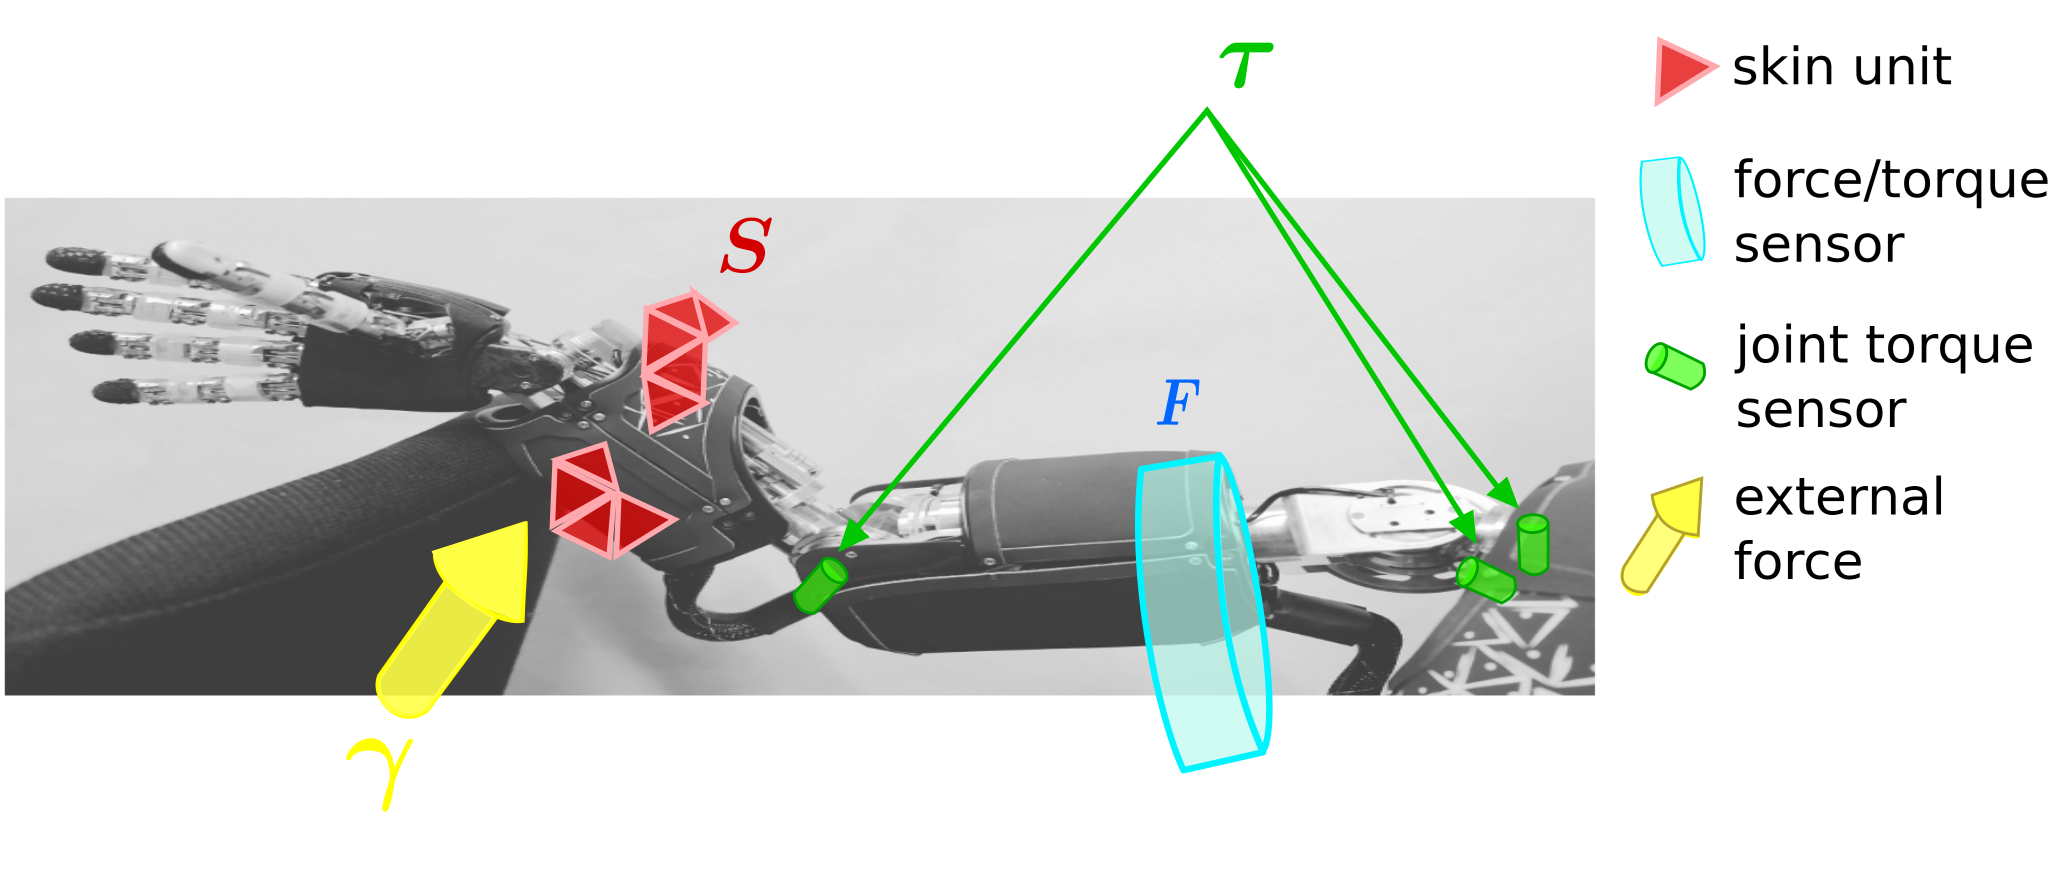
\includegraphics[width=.5\columnwidth]{robertoIROS/fig/concept_gray}		
  \caption{Illustration of the force/torque and tactile sensors involved during a contact of the robot arm with the environment.}
  \label{fig:robIROS_concept}
\end{figure}
%

%%%%%%%%%%%%%%%%%%%%%%%%%%%%%%%%%%%%%%%%%%%%%%%%%%%%%%%%%%%%%%%%%%%%%%%%%%%%%%%%

\section{Control with Tactile Sensing} 
\label{sec:robIROS_method}



In this section, we present our proposed approach to learning inverse dynamics with contacts.
We first formalize the problem as learning a mixture-of-experts model.
Then we detail how to implement Gaussian processes as the corresponding experts.


\subsection{Learning a Mixture-of-Contacts}



	When learning the inverse dynamics with contacts (\eq\eqref{eq:robIROS_tau_contact}), we assume that the (contact-free) inverse dynamics from \eq\eqref{eq:robIROS_tau_nocontact} can be computed precisely, either from an analytical model or from a learned model~\cite{Nguyen-Tuong2011}.
    %
    In our experiments, we employ a learned GP model for this purpose.
    The reason for this choice are the unmodeled dynamics $\epsilon\,(\q,\dq,\ddq)$, which introduce substantial errors even in absence of contacts.
	%
	As a result of this contact-free inverse dynamics, only the model of the additional term of the external forces $\color{darkgreen}{\sum_{i \in\mathcal{C}} {\jacobian_i(\q)}\T \extForces_i}$ has to be learned.
    In this paper, we consider a robot that is provided with skin measurements~$\skinInput$ from the tactile sensors, force measurements~$\ftsForces$ from the force torque sensors (FTS) and the applied torques~$\torques$.
    A visual representation of these relevant components is shown in \fig\ref{fig:robIROS_concept}.
	Predicting the external forces $\color{darkgreen}{\sum_{i \in\mathcal{C}} {\jacobian_i(\q)}\T \extForces_i}$ can be formalized as the regression task
  	%
	\begin{align}
		\outputMatrix = \regressionNo(\inputMatrix) + \epsilon\,,
		\label{eq:generic_regression_noise}
	\end{align}
	%    
	where $\outputMatrix = \textcolor{darkgreen}{\sum_{i \in\mathcal{C}} {\jacobian_i(\q)}\T \extForces_i}$ and  $\inputMatrix = [\q, \skinInput,\ftsForces]$ are the inputs. 
	Additionally, $\epsilon$ is an i.i.d. Gaussian measurement noise with mean~$0$ and variance~$\sigma_n$.
	Therefore, our regression problem is phrased as
  	%
	\begin{align}
		\outputMatrix =\textcolor{darkgreen}{\sum_{i \in\mathcal{C}} {\jacobian_i(\q)}\T \extForces_i}  = \regressionNo([\q, \skinInput,\ftsForces]) + \epsilon\,.
		\label{eq:robIROS_regression}
	\end{align}
	%    
	%
	It is necessary to consider the skin as an input~$\skinInput$ since contacts with different parts of the body lead to different effects in the dynamics.
	Intuitively, $\skinInput$ is required to identify the position of the contact.
	The force/torque measurements~$\ftsForces$ could be avoided if we were interested in learning contacts that do not change between training and test time, which would restrict us to dealing with static objects, such as a rigid floor, walls or stationary obstacles.
	However, as this assumption is limiting, we include the force/torque measurements~$\ftsForces$ in our model.

	The resulting regression of \eq\eqref{eq:robIROS_regression} is a highly complex task, due to the extremely high-dimensional space of the input $\inputMatrix \in \inputSpace$ (the skin measurements~$\skinInput$ alone account for hundreds of dimensions) and nonlinearity.
    We tackle this problem by rephrasing it as a problem of learning a mixture-of-experts model (``mixture of contacts'' in our case).
	With this model, we decompose \eq\eqref{eq:robIROS_regression} as
	%
	\begin{align}
		\textcolor{darkgreen}{\sum_{i \in\mathcal{C}} {\jacobian_i(\q)}\T \extForces_i}  = \sum_{j\in\mathcal{J}} f_j([\q, \ftsForces]) + \epsilon\,,
		\label{eq:robIROS_expertofmixtureregression}
	\end{align}
	%    
	where $\mathcal{J}$ is the set of active experts~$f_j$.
    %, which depends from $[\q, \skinInput]$.
	Note that the skin input~$\skinInput$ is no longer explicitly part of the inputs of the experts. 
    Hence, each single expert~$f_j$ is now sufficiently low-dimensional to be modeled independently, but at the same time the possibility of summing the contribution of each contact allows to account for complex behaviors.
    As single expert~$f_j$ we propose to use Gaussian processes mapping $[\q, \ftsForces] \mapsto {\jacobian_j(\q)}\T \extForces_j$.
    Detailed information regarding the GP models and their training are given in the next subsection.
    The purpose of the gating network is then to select the experts that are currently active and to add their contributions.    
    An illustration of our approach is shown in \fig\ref{fig:robIROS_model}.
	For mixture-of-experts models it is required to design a suitable gating network that activates the relevant experts.
    In our case, this gating network can be considered a classifier $\mathcal{J} = g(\q, \skinInput,\ftsForces)$ that selects which contact is currently ongoing.
	For simple tasks, this gating network can be designed using heuristics (e.g., using thresholds on the activation of the tactile sensors). 
    Alternatively, for more complex systems an approach based on machine learning is more suitable. 
    %In the experimental section we also evaluate the learning of such gating network.
	%This automatic design is increasingly helpful for high number of skin sensor ($>1000$), where the manual design became increasingly complex.

%\todo[inline]{How do you define the experts? And how many do you need? Not mentioned.}

%\todo[inline,color=yellow]{Make sure the section headings are consistently capitalized.}

	%
	\begin{figure}[t]
		\centering
		\includegraphics[width =.58\linewidth]{robertoIROS/fig/diagram_2.pdf}
		\caption{Our approach extends existing inverse dynamics without contacts by learning many contact models which serve as correction terms under different contacts type. The decision of which contact model to activate is taken by a gating network based on the skin measurements~$\skinInput$, the force torque sensors~$\ftsForces$ and the current state $\q, \dq, \ddq$.}
		\label{fig:robIROS_model}
	\end{figure}
	%

%=============================================================


\subsection{Gaussian Processes as Expert Models}
%\todo[inline]{Introduce GPs only in the context of IDM: distribution over IDMs (instead of "function"), RBD as prior mean, define X and Y in this context immediately.}
	Gaussian Processes~\cite{Rasmussen2006} are a state-of-the-art regression method.
	They have been used in robotics to learn dynamics models~\cite{Deisenroth2012} and for control~\cite{Deisenroth2014}.
    %
    In the context of this paper, a GP is a distribution over inverse dynamics models 
	%
	\begin{align}
		f \sim \GP \left( m_f,k_f \right) \,,
	\end{align}
	%
	fully defined by a prior mean~$m_f$ and a covariance function~$k_f$.
	In our experiments, we choose as prior mean $m_f \equiv \torques_\text{RBD}$ and as covariance function~$k_f$ the squared exponential with automatic relevance determination and Gaussian noise:
    %
	\begin{align}
		{k(\vec x_p,\vec x_q)} &= \sigma_f^2\exp\left(\!-\!\tfrac{1}{2}(\vec x_p\! -\!\vec x_q)^T {\mat \Lambda\inv} (\vec x_p \!-\! \vec x_q)\right) \!+\! \sigma_w^2\delta_{pq}
		\label{sec:GP:cov:SE}
	\end{align}
	%
	where ${\mat \Lambda}=\diag([l^2_1,...,l^2_D])$ and $\delta_{pq}$ is the Kronecker delta (which is one if $p=q$ and zero otherwise). Here, $l_i$ are the characteristic length-scales, $\sigma^2_f$ is the variance of the latent function $f(\cdot)$ and $\sigma^2_w$ the noise variance. 
 %   The purpose of $\sigma_w^2\delta_{pq}$ is to model (and identify) the presence of the Gaussian noise~$\epsilon$.
    In our experiments, when learning contact models, the input is defined as $\parameters = [\q,\ftsForces]$ and the output (observations) is $\vec y = \torques$ are the torques.
    Hence, given $n$ training inputs $\mat X=[\parameters_1,...,\parameters_n]$ and corresponding training targets $\mat y=[ y_1,..., y_n]$, we define the training data set $\dataset = \{\mat X,\mat y\}$. 
    % training
Training the GP corresponds to finding good hyperparameters $\parameters = [l_i, \sigma_f, \sigma_w]$, which is done by the standard procedure of maximizing the marginal likelihood~\cite{Rasmussen2006}.   
    
% predictive distribution    
    The GP yields the predictive distribution over torques for a new input $\vec x_* = [\vec q_*, \mat F_*]$
	%
	\begin{align*}
		&\prob(\vec y|\dataset,\parameters_*) = \gauss{\mu(\parameters_*)}{\sigma^2(\parameters_*)}\,, 
		%\label{eq:one-step prediction distr}
	\end{align*}
	%
	where the mean~$\mu(\parameters_*)$ and the variance~$\sigma^2(\parameters_*)$ are 
	%
	\begin{align*}
		&\mu(\parameters_*) = \vec k^T_*\vec K^{-1} \mat y\,,\quad \sigma^2(\parameters_*) = k_{**}-\vec k^T_*\mat K^{-1}\vec k_*\,.
		%\label{eq:one-step prediction mean and covariance}
		%\label{eq:one-step prediction cov}
	\end{align*}
	%
	%% all the stuff from the equations
	The entries of the matrix $\vec K$ are  $K_{ij}= k(\parameters_i,\parameters_j)$, and we define $k_{**}=k(\parameters,\parameters)$ and $\vec k_{*}=k(\vec X,\parameters)$. 

%=============================================================

\subsection{Controlling the Contacts}

In the case of no contacts $\mathcal{C}=\{0\}$ we can define the Task-space Nonlinear Feedforward Control:
%
\begin{align}
	\vec u = \torques_\text{RBD}\,,
\end{align}
%
where the~$\torques_\text{RBD}$ is computed from the rigid body inverse dynamics (or a learned model of it).
Often an additional PD feedback controller is added to compensate for noise and inaccuracies in the dynamics, such that
%
\begin{align}
	\vec u = \torques_\text{RBD} + \underbrace{K_P \left(\q^{\text{des}}-\q\right) + K_D \left(\dq^{\text{des}} - \dq\right)}_{\torques_\textit{PD}}\,.
\end{align}
%
Intuitively, the magnitude of the torques contribution from the PD controller~$\torques_\textit{PD}$ can be used to measure the goodness of our inverse dynamics model.
Accurate inverse dynamics model will only need small corrections by the feedback controller, while inaccurate models will rely more heavily on it.
In case of inaccurate models increasing the PD gains can still lead to acceptable tracking performance at the expense of safety.
However, with unforeseen obstacles, high gains can lead to both damages to the robot's hardware and the obstacle itself.

%%%%%%%%%%%%%%%%%%%%%%%%%%%%%%%%%%%%%%%%%%%%%%%%%%%%%%%%%%%%%%%%%%%%%%%%%%%%%%%%

\section{Experimental Results}
\label{sec:robIROS_results}

In this section we present the experiments we will conduct. Two different tracking tasks in presence of external contacts will be investigated.
First, we will demonstrate that a controller using a learned inverse dynamics model can be used to compensate for contact forces and that the tracking performance of a tracking controller will be improved.
In a second experiment, we will demonstrate that the same inverse dynamics model can also be used to avoid an obstacle and gently slide along it. 



\subsection{Experimental Setting}

	Both experimental evaluations are performed on a real \robot{} humanoid robot~\cite{Natale2013}.
    The \robot{} possess 53 degrees of freedom and is 104 cm tall for 24 kg of weight.
    Four 6-axis force/torque sensors placed are proximally in the middle of legs and arms.
    Additionally, artificial skin consisting of more than 2000 tactile sensors are mounted on the robot covers~\cite{Cannata2008}.
 	%
    In our experiments, we control 5 DoF of the \robot{} arm: shoulder pitch, roll and jaw, elbow and wrist pronosupination. 
    Therefore $\q \in \R^5$, $\dq \in \R^5$, $\ddq \in \R^5$, $\torques \in \R^5$ and $\ftsForces \in \R^3$ resulting in learning the mapping $\inputMatrix \in \R^{18} \mapsto \outputMatrix \in \R^5$.
    The skin input~$\skinInput$ from the forearm consists of 270 sensors.
    

\subsection{Pushing Obstacles}
	%
    \begin{wrapfigure}{r}{0.2\columnwidth}
	%\begin{figure}[t]
		\centering
		\includegraphics[width=.99\linewidth]{robertoIROS/fig/taskPush}
		\caption{\textbf{Pushing Obstacles. }}
		\label{fig:pushSetup}
	%\end{figure}
    \end{wrapfigure}
	%

    For classical controllers, when an obstruction occur, the rigid body inverse dynamics does not account for this variation. 
    As a result, the tracking error increase and the contribution of the PD feedback controller increases to compensate for this tracking error.
	In this scenario we demonstrate that it is possible to use a learned model to improve the tracking accuracy when unforeseen and unknown obstruction are encountered along the path.
    Additionally, we show that such learned dynamics allows to reduce the PD gains to achieve an increased safety, without loss in tracking accuracy.
	
    We first consider the \robot{} following a pre-defined trajectory with the left arm.
    Following, we repeat the same trajectory, but this time with an unforeseen obstruction. 

    To compare the performance of our learned inverse dynamics we first analyze the tracking error introduced by the obstruction.
    
%%%%%%%%%%%%%%%%%%%%%%%%%%%%%%%%%%%%%%%%%%%%%%%%%%%%%%%%%%%%%%%%%%%%%%%%%%%%%%%%

	
%%%%%%%%%%%%%%%%%%%%%%%%%%%%%%%%%%%%%%%%%%%%%%%%%%%%%%%%%%%%%%%%%%%%%%%%%%%%%%%%


%%%%%%%%%%%%%%%%%%%%%%%%%%%%%%%%%%%%%%%%


\bibliographystyle{plain}
\bibliography{manuscript}

\end{document}

%%% Local Variables:
%%% mode: latex
%%% TeX-master: t
%%% save-place: t
%%% End:
